\documentclass[12pt,reqno,a4paper,oneside]{article}

\usepackage{amsfonts, amsmath,
	        amssymb, amsthm}  % Fontes e símbolos matemáticos da AMS.
\usepackage{graphicx}         % Importação de gráficos.
\usepackage{subfig}
\usepackage[brazil]{babel}    % Idioma português (Brasil) como padrão.
\usepackage[utf8]{inputenc}   % Codificação UTF-8.
%\usepackage{natbib}           % Para citações.
%\usepackage{cite}             % Idem.

\usepackage{bm}          % Equações em negrito com qualidade superior.
\usepackage{booktabs}    % Edição de linhas de tabelas.
\usepackage{caption}     % Edição do texto dos títulos de tabelas.
\usepackage{color}       % Edição de cores.
\usepackage{indentfirst} % Indentará sempre o 1º parágrafo de cada seção do relatório.
%\usepackage{enumitem}   % Edição mais elaborada de listas
                         % Conflito com ambiente "enumerate" no beamer!.
%\usepackage{hyperref}   % Criação de "hyperlinks".
\usepackage{multirow}    % Para obter uma célula com uma coluna e várias linhas.
\usepackage{ragged2e}    % Opções de alinhamento do texto.

%\usepackage[FIGTOPCAP]{subfigure} % Acesso a figuras dentro de pastas.

\usepackage[top=2cm, bottom=2cm,
            left=2cm, right=2cm]{geometry} % Margens do texto.

\captionsetup{justification = centering} % Centraliza os títulos das tabelas.

% Símbolo matemático para independência entre variáveis aleatórias:

\newcommand\indep{\protect\mathpalette{\protect\independenT}{\perp}}\def\independenT#1#2{\mathrel{\rlap{$#1#2$}\mkern2mu{#1#2}}}

\begin{document}

\title{\huge Relatório do Trabalho de\\
	Estatística Bayesiana I}
\author{\\
	\\
	\huge Mistura de Normais\\
	\huge com Variância Contaminada\\
	\\
	\\
	\\
	\\
	\Large Caio Balieiro\\
	\Large Taiguara Melo Tupinambás\\
	\Large Walmir dos Reis Miranda Filho\\
	\\
	\\
	\\
	\\
	\Large Prof. Dani Gamerman\\
	\Large Profª Rosangela Helena Loschi\\
	\\
	\\
	\\
	\\
	\\
	Programa de Pós-Graduação em Estatística\\
	Instituto de Ciências Exatas\\
	Universidade Federal de Minas Gerais\\
	\\
	\\
	\\
	\\
	\\
	\\}
\date{Belo Horizonte, 2 de dezembro de 2019}
\maketitle

\newpage

\section{Introdução}

O presente trabalho tem como objetivo obter, dada uma densidade \textit{a posteriori} conjunta dos parâmetros de um modelo probabilístico para uma amostra previamente observada, as densidades \textit{a posteriori} marginais de cada parâmetro, bem como as estatísticas de média; variância; assimetria e curtose associadas, a partir da implementação de três métodos numéricos, a saber: (i) integração via quadratura de Riemann; (ii) reamostragem por importância sequencial (em inglês, \textit{Sequential Importance Resampling}, ou SIR); e (iii) integração via Monte Carlo em cadeias de Markov (em inglês, \textit{Markov Chain Monte Carlo}, ou MCMC) com inovações dadas pelo algoritmo de Metropolis-Hastings (MH).

Para o modelo que gerou a amostra observada, será pressuposto que sua especificação é dada por uma mistura finita de normais. Sejam $X_{1}, \ldots, X_{n}$ amostras aleatórias independentes, condicionalmente a um vetor de parâmetros $\bm{\theta} = (\mu, \sigma^2, \nu)$, e identicamente distribuídas com função densidade dada por
\begin{equation}\label{eq:dist_am}
f(x | \mu, \sigma^2, \nu) = \nu \phi(x | \mu, 100 \sigma^2) + (1 - \nu) \phi(x | \mu, \sigma^2), \ x \in \mathbb{R},
\end{equation}
\noindent onde $\phi(x | \mu, \sigma^2) = (2\pi\sigma^2)^{-1} \exp[-(x - \mu)^2/(2\sigma^2)]$ denota a função densidade da distribuição normal com média $\mu$ e variância $\sigma^2$ avaliada no ponto $x$. Para o suporte de cada parâmetro, tem-se que $\mu \in \mathbb{R}, \sigma^2 \in \mathbb{R}_+$ e $\nu \in (0,1)$.

A mistura finita descrita em \eqref{eq:dist_am} possui duas componentes normais que diferem nas respectivas variâncias: para a primeira componente, o valor é 100 vezes o da segunda. Desta forma, tem-se uma mistura finita de normais com variância \textit{contaminada}.

Para os parâmetros $\mu$, $\sigma^2$ e $\nu$, será pressuposto que cada um segue uma distribuição \textit{a priori} predeterminada: $\mu | \sigma^2 \sim{N} (m, V \sigma^2)$, onde $N(\cdot)$ denota a distribuição normal com média $m \in \mathbb{R}$ e variância $V \sigma^2$, $V > 0$; $\sigma^2 \sim{GI} (a,d)$, onde $GI(\cdot)$ denota a distribuição gama inversa com parâmetros de forma $a > 0$ e de taxa $d > 0$ (inverso da escala); e $\nu \sim{U}(0,1)$, a distribuição uniforme contínua padrão.

Para gerar uma amostra aleatória do modelo em $\eqref{eq:dist_am}$, foi utilizada uma representação hierárquica (Lachos \textit{et al.}, 2013)\cite{Lachos2013} tal que
\begin{equation}
X_i | \mu, \sigma^2, U_{i} = u_i \sim{N}(\mu, \sigma^2 u_i^{-1}), \quad U_i | \mu \sim{p_d}(1,100) : P(U_i = 100) = \nu. \label{eq:hier}
\end{equation}
\noindent onde $p_d(a,b)$ denota uma função de probabilidade (discreta) que atribui massa probabilística apenas aos pontos $a$ e $b$.

A partir do produto entre a função de verossimilhança $f(\bm{x} | \mu, \sigma^2, \nu)$ para uma amostra $\bm{x} = (x_1, \ldots, x_n)$ gerada através da representação hierárquica em \eqref{eq:hier} e das densidades \textit{a priori} para cada parâmetro do modelo, obtém-se o núcleo (em inglês, \textit{kernel}) da densidade \textit{a posteriori} conjunta $p(\mu, \sigma^2, \nu | \bm{x})$. Como a expressão da densidade \textit{a posteriori} possui uma constante de proporcionalidade $f(x_1, \ldots, x_n) = f(\bm{x})$ não facilmente calculável, mas que não depende dos parâmetros, pode-se usar o núcleo daquela para inferir sobre cada um dos parâmetros. No modelo de mistura finita de duas componentes normais com variância contaminada, temos que
\begin{align}
p(\mu, \sigma^2, \nu | \bm{x})
&= \dfrac{f(\bm{x} | \mu, \sigma^2, \nu) \times p(\mu, \sigma^2, \nu)}{f(\bm{x})} \propto \prod_{i=1}^{n} f(x_i) \times p(\mu | \sigma^2) \times p(\sigma^2) \times p(\nu) \nonumber\\
&\propto \prod_{i=1}^{n} \left[ \nu \phi(x_i | \mu, 100 \sigma^2) + (1 - \nu) \phi(x_i | \mu, \sigma^2) \right] \times \nonumber \\
&\times \phi(\mu | m, V \sigma^2) \times \dfrac{d^a}{\Gamma(a)} \left(\dfrac{1}{\sigma^2}\right)^{a + 1} \exp\left(-\dfrac{d}{\sigma^2}\right) \nonumber \\
&\propto \left(\dfrac{1}{\sigma^2}\right)^{(n + 1)/2 + a + 1} \exp\left\{-\dfrac{\left[(\mu - m)^2 / (2V) + d\right]}{\sigma^2}\right\} \times \textrm{A}(\bm{x} | \mu, \sigma^2, \nu), \label{eq:dist_post}
\end{align}
onde
\begin{equation*}
\textrm{A}(\bm{x} | \mu, \sigma^2, \nu) = \prod_{i=1}^{n} \left\{  \dfrac{\nu}{10} \exp\left[-\dfrac{(x_i - \mu)^2}{200\sigma^2}\right] + (1 - \nu) \exp\left[-\dfrac{(x_i - \mu)^2}{2\sigma^2}\right] \right\}.
\end{equation*}

Evidentemente, trabalhar diretamente com o lado direito em \eqref{eq:dist_post} não é computacionalmente agradável, uma vez que este é um produto de várias quantidades sempre menores do que 1, muitas delas próximas de 0, o que pode levar a problemas de aproximação numérica. Desta forma, sempre que for necessário calcular o núcleo da \textit{posteriori}, dada uma amostra, inicialmente será tomada a soma do logaritmo de todos as quantidades que compõem este produto e só depois esta mesma soma será exponenciada. Dependendo do quão negativa for a soma (o logaritmo de termos entre 0 e 1 é sempre negativo), quando exponenciada ela pode ou não ser menor que o mínimo aceito pelo \textit{R}, se tornando igual a 0.

Logo, na geração da amostra $\bm{x}$ deve-se escolher valores de $\mu$, $\sigma^2$ e $\nu$ tais que o núcleo de $p(\mu, \sigma^2, \nu | \bm{x})$ não seja numericamente nulo para os verdadeiros valores dos parâmetros. Considerando o uso da linguagem de programação \textit{R} (R Core Team, 2019)\cite{RCoreTeam2019}, esta escolha não é difícil. Na versão 3.5.3, o menor valor inteiro que pode ser tomado como argumento da função \verb|exp()| do \textit{R} é $-745$. Desta forma, basta tomar $\mu$, $\sigma^2$ e $\nu$ tais que o logaritmo do lado direito em \eqref{eq:dist_post} seja maior do que $-745$.

Para o presente trabalho, foram considerados uma amostra de tamanho $n=500$ (Figura \ref{fig:sample_n}) da mistura finita de normais com variância contaminada parametrizada de tal forma que $\mu = 11$; $\sigma^2 = 0.64$ e $\nu = 0.2$, com hiperparâmetros $m = 11$; $V = 1$; $a = 7$ e $d = 4$ nas distribuições \textit{a priori}. Fixada uma semente aleatória, para a amostra gerada a partir dos valores citados, o logaritmo do núcleo da densidade \textit{a posteriori} é igual a $-518.9061$, cuja exponencial é aproximadamente igual a $4.385 \times 10^{-226}$.

\begin{figure}[htb]
	\centering
	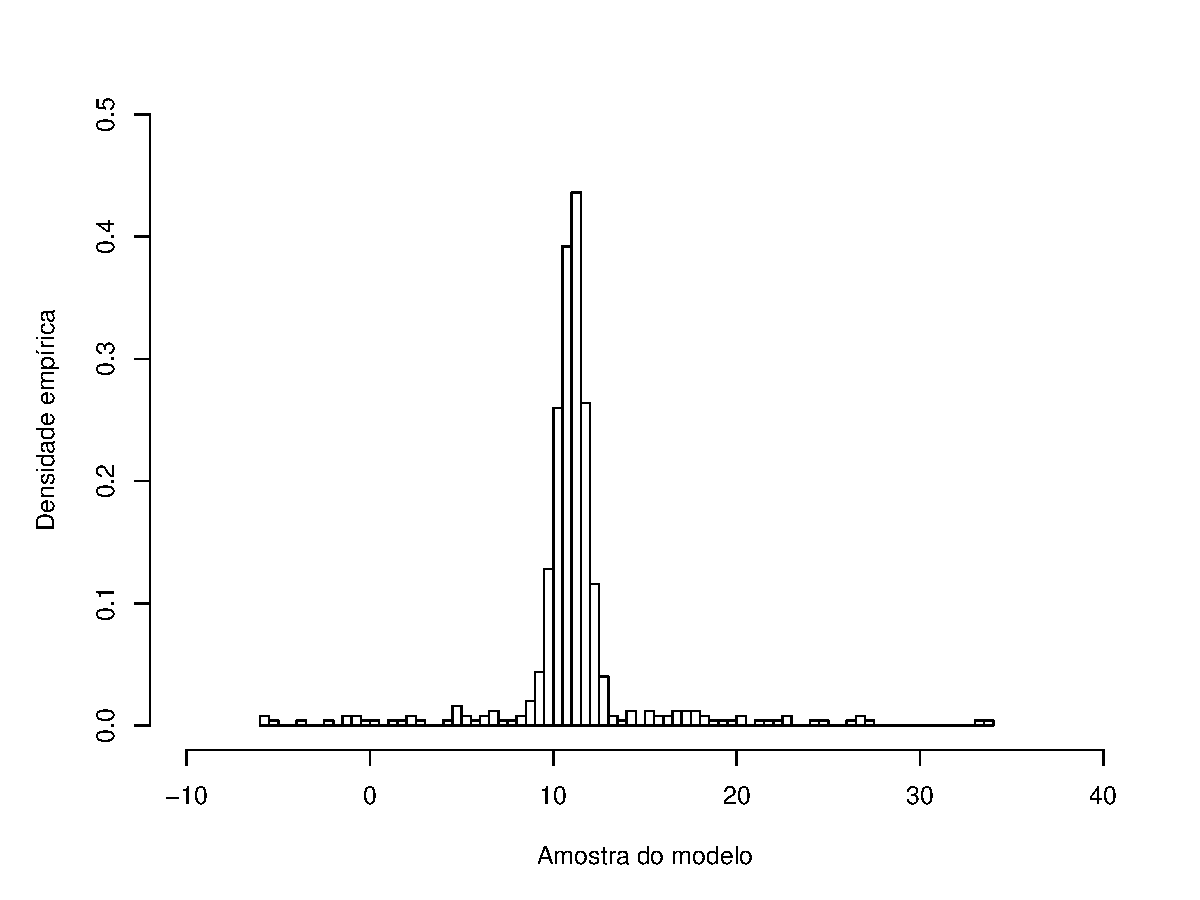
\includegraphics[scale=0.8]{figuras/amostra_n.pdf}
	\caption{Histograma da amostra gerada do modelo}
	\label{fig:sample_n}
\end{figure}

Como não se tem uma expressão fechada para $p(\mu, \sigma^2, \nu | \bm{x})$, mas apenas de seu núcleo, para obter as densidades \textit{a posteriori} marginais de $\mu$, $\sigma^2$ e $\nu$ dado $\bm{x}$, bem como as estatísticas associadas a cada uma delas, é necessário aproximá-las por algum método numérico. Na seções \ref{quarie}, é apresentado o primeiro dos três métodos considerados: a integração via quadratura de Riemann. Por sua vez, na seção \ref{sir} é descrito o método SIR. Por fim, na seção \ref{mcmc}, é retratada a integração via MCMC com inovações MH. Todos os métodos serão testados e comparados no contexto do modelo exposto acima. Na seção \ref{consfin}, são resumidos os resultados obtidos para os três métodos, bem como é feita uma avaliação comparativa da qualidade de sua convergência.

Antes de implementar cada um dos métodos numéricos, foram feitos três gráficos (Figuras \ref{fig:maspro_mu} a \ref{fig:maspro_nu}) do núcleo de $p(\mu, \sigma^2, \nu | \bm{x})$ quando se varia um dos três parâmetros e os outros dois são mantidos fixos nos respectivos valores verdadeiros pressupostos para o modelo que gerou a amostra. Tais gráficos permitem dizer, para cada parâmetro, quais são os intervalos do suporte correspondente que concentram praticamente toda a massa probabilística da densidade \textit{a posteriori} marginal associada, ainda que as densidades calculadas sejam válidas apenas quando os outros dois parâmetros são fixados em valores arbitrários. Esta informação será útil para definir os intervalos de integração na quadratura de Riemann e a matriz de covariância da distribuição proposta nos métodos SIR e MCMC-MH para aproximação das densidades \textit{a posteriori} marginais verdadeiras.

\begin{figure}[htb]%
	\centering
	\subfloat[$I_{\mu} = (10.85,11.13)$, dados $\sigma^2 = 0.64, \nu = 0.2$]{
		{
			\label{fig:maspro_mu}
			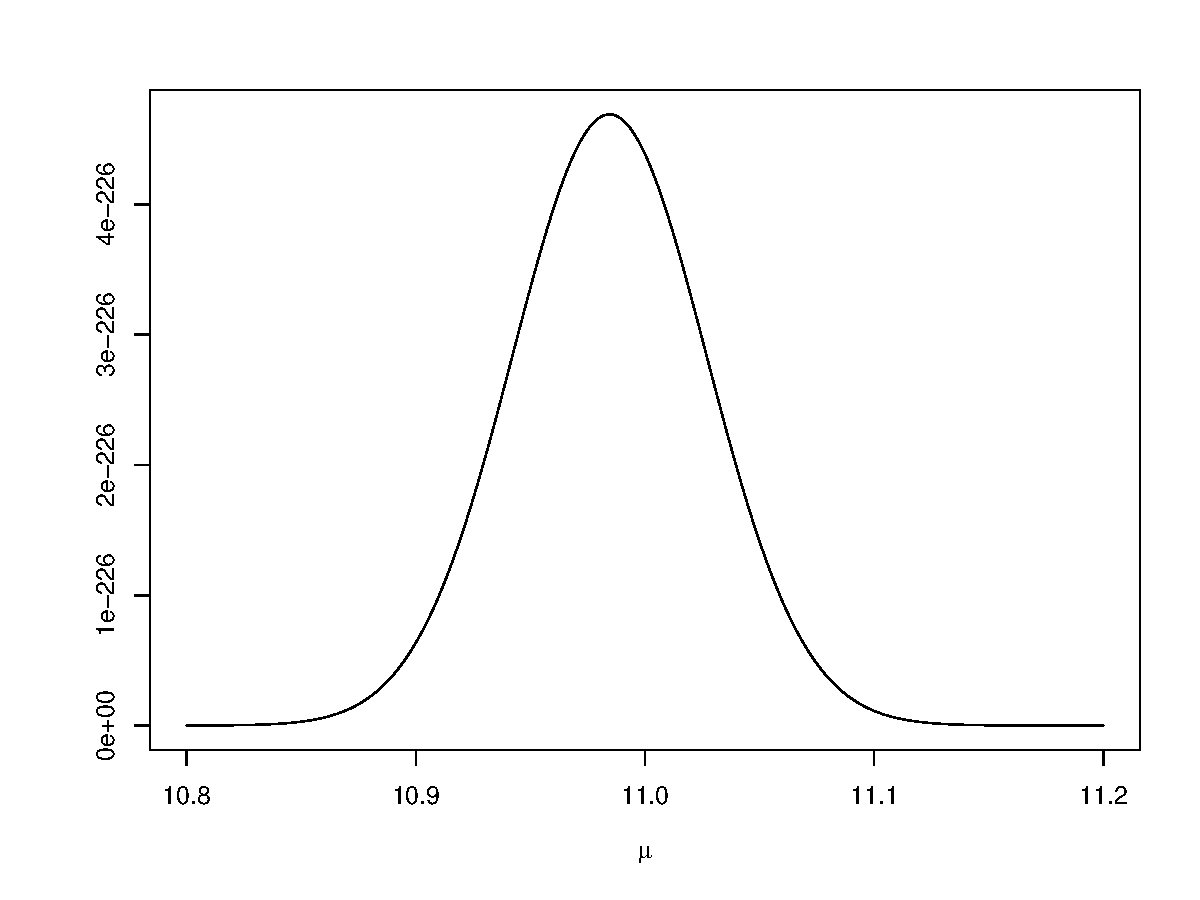
\includegraphics[scale=0.4]{figuras/maspro_mu.pdf}}}%
	\qquad
	\subfloat[$I_{\sigma^2} = (0.48, 0.78)$, dados $\mu = 11, \nu = 0.2$]{
		{
			\label{fig:maspro_s2}
			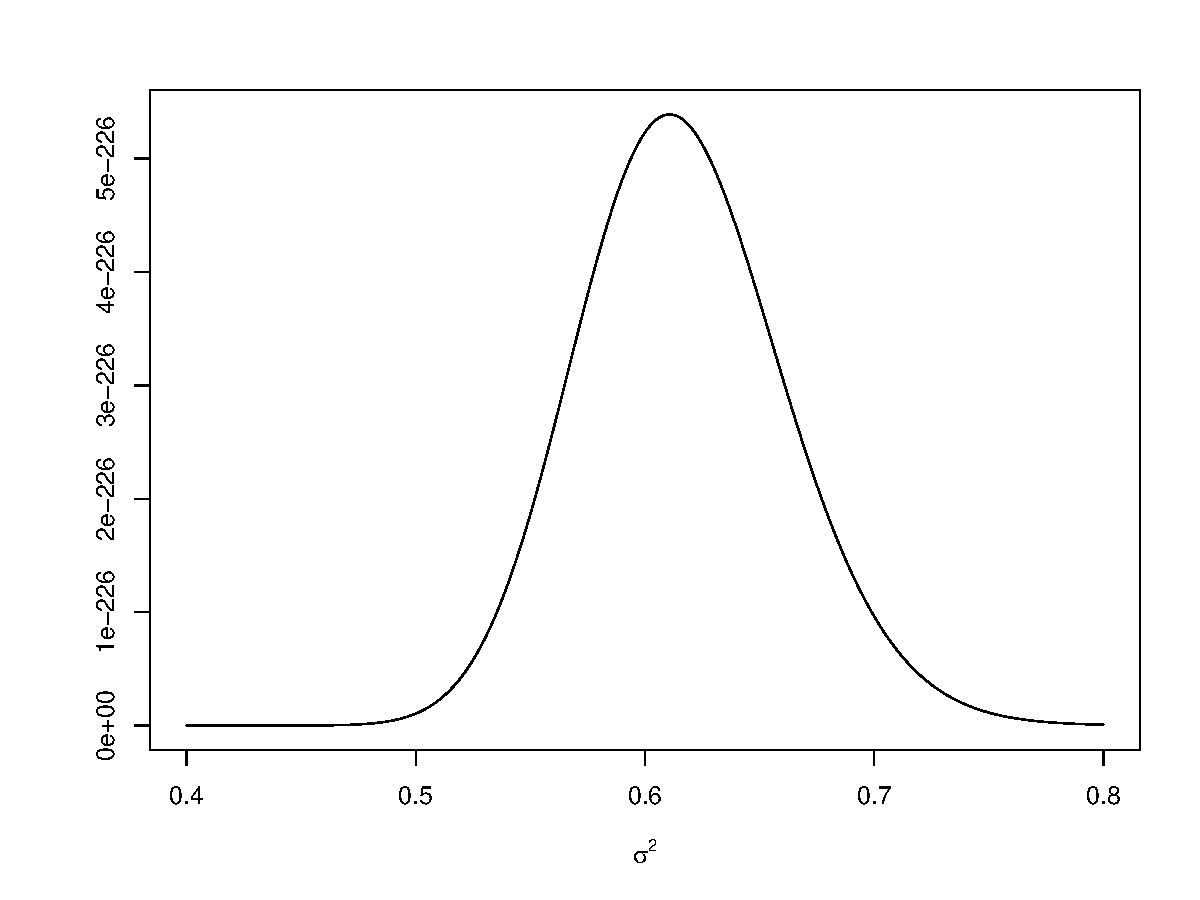
\includegraphics[scale=0.4]{figuras/maspro_s2.pdf}}}%
	\subfloat[$I_{\nu} = (0.13, 0.26)$ dados $\mu = 11, \sigma^2 = 0.64$]{
		{
			\label{fig:maspro_nu}
			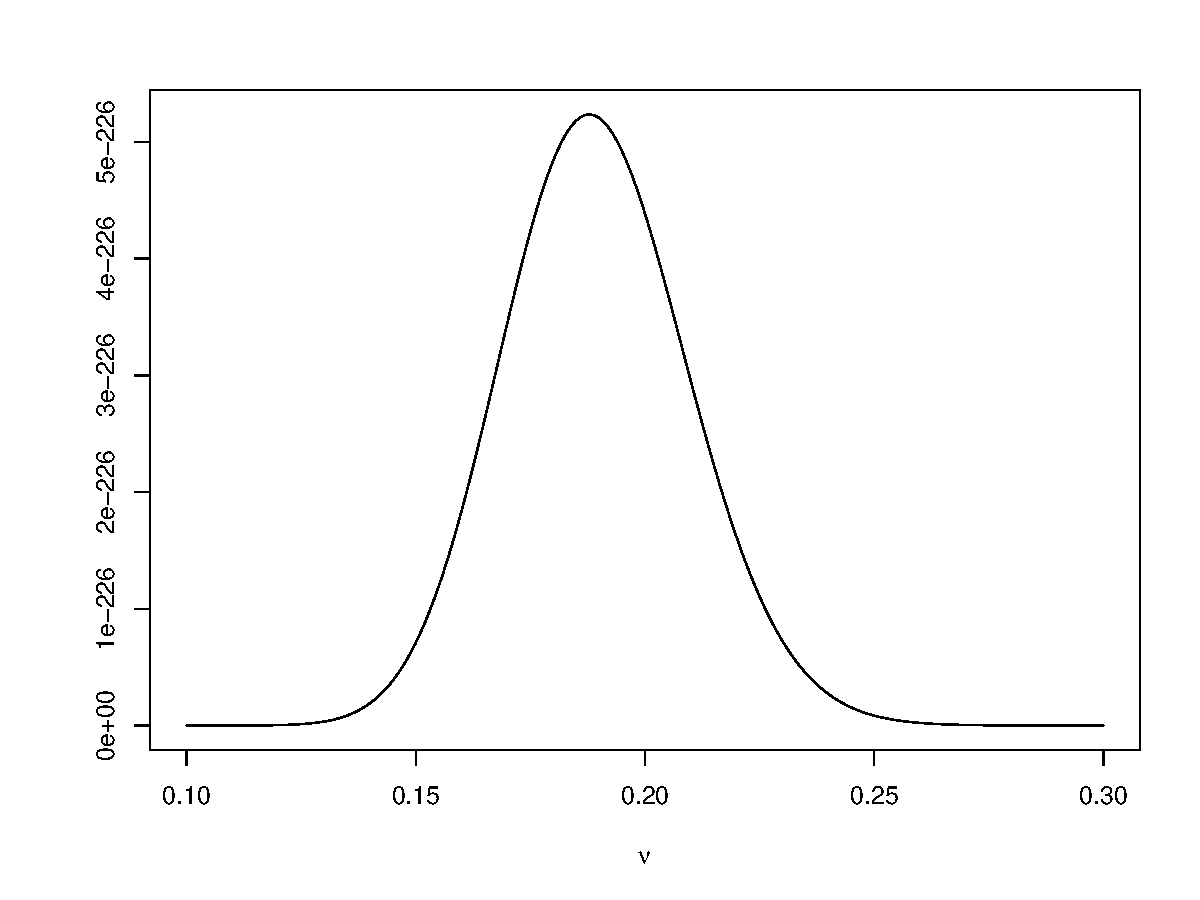
\includegraphics[scale=0.4]{figuras/maspro_nu.pdf}}}%
	\caption{Intervalos de massa probabilística para cada parâmetro (variável aleatória) do núcleo de $p(\mu, \sigma^2, \nu | \bm{x})$}%
\end{figure}

\newpage
\section{Quadratura de Riemann}\label{quarie}

Em problemas multidimensionais, a densidade marginal correspondente a cada variável aleatória para a qual se deseja fazer inferência é obtida integrando a densidade conjunta sobre as demais. Frequentemente, o cálculo das integrais pode ser difícil ou mesmo impossível analiticamente. No caso de uma densidade \textit{a posteriori} conjunta deve-se aproximar algumas das, ou todas as, integrais associadas a cada densidade \textit{a posteriori} marginal de interesse por métodos numéricos, os quais podem ser determinísticos ou estocásticos. Neste presente trabalho, isto será feito para todos os 3 parâmetros do modelo de mistura finita de normais com variância contaminada.

Dentre os métodos determinísticos mais usuais, para a aproximação das integrais correspondentes às densidades \textit{a posteriori} marginais de $\mu$, $\sigma^2$ e $\nu$, será utilizado o método da quadratura de Riemann, um caso particular e o mais simples da família das \textit{fórmulas de Newton-Cotes} (Chapra, 2015)\cite{Chapra2015}, as quais substituem o verdadeiro integrando por uma aproximação polinomial dentro de cada subintervalo contido no intervalo de integração. Na quadratura de Riemann, o integrando avaliado em cada subintervalo é aproximado por uma função constante avaliada no limite inferior (ou superior) do mesmo subintervalo.

Aproximações polinomiais com nós igualmente espaçados a cada subintervalo, como as regras de quadratura do Trapézio (grau 1) ou de Simpson (grau 2), obtém resultados com menor erro do que a quadratura de Riemann. Quando o grau da aproximação polinomial tende ao infinito, a quadratura converge para o verdadeiro valor da integral. Porém, em problemas de dimensão igual a 2 ou superior, usar aproximações polinomiais com nós torna-se muito custoso computacionalmente, uma vez que temos três ou mais termos na soma que aproximará a integral para cada dimensão. Por esta razão, escolheu-se a quadratura de Riemann para obter densidades \textit{a posteriori} marginais de $\mu$, $\sigma^2$ e $\nu$, pois esta regra possui um único termo na soma aproximadora, facilitando a programação das rotinas iterativas associadas. Em uma dada aproximação, o mesmo número de intervalos será usado para todas as dimensões.

Antes de aproximar as densidades \textit{a posteriori} marginais de cada parâmetro, é necessário aproximar o inverso da constante de proporcionalidade. Dados três parâmetros $(\alpha_1, \alpha_2, \alpha_3)$ e uma amostra dos dados $\bm{y}$ quaisquer, suponha que se deseja aproximar a densidade \textit{a posteriori} marginal de $\alpha_3$ dados os pontos $r_i, s_j, t_k$ da grade formada por todos os subintervalos de integração, $i, j, k \in \{1, \ldots, L\}$. Temos pela quadratura de Riemann que
\begin{align}
p(\alpha_3 | \bm{y})
&= \iint p(\alpha_1, \alpha_2, \alpha_3 | \bm{y}) d\alpha_1 d\alpha_2 \nonumber \\
\Rightarrow p(t_k | \bm{y})
&= \iint p(\alpha_1, \alpha_2, t_k | \bm{y}) d\alpha_1 d\alpha_2 \approx \sum_{i=1}^{L} \sum_{j=1}^{L} p(r_i, s_j, t_k | \bm{y}) \Delta_i \Delta_j \nonumber \\
&= \sum_{i=1}^{L} \sum_{j=1}^{L} c \cdot h(r_i, s_j, t_k | \bm{y}) \Delta_i \Delta_j. \label{eq:dpm_riem}
\end{align}

Como $c$, a constante de proporcionalidade, é dada pelo inverso da densidade \textit{a priori} preditiva $f(\bm{y})$, a qual é obtida integrando-se em todo o espaço paramétrico o produto entre a função de verossimilhança $f(\bm{y} | \alpha_1, \alpha_2, \alpha_3)$ e as densidades (ou funções de probabilidade) \textit{a priori} para $\alpha_1$, $\alpha_2$ e $\alpha_3$, também é possível aproximar $c$ pela quadratura de Riemann. Neste caso, $c^{-1} \approx \sum_{i=1}^{L} \sum_{j=1}^{L} \sum_{k=1}^{L} h(r_i, s_j, t_k | \bm{y}) \Delta_i \Delta_j \Delta_k$. Com o valor aproximado para $c$, é possível calcular \eqref{eq:dpm_riem} nos limites superior e inferior de todos os subintervalos de um dado parâmetro e enfim obter uma aproximação da densidade \emph{a posteriori} marginal deste mesmo parâmetro através de uma curva gráfica que liga todos os valores calculados. Evidentemente, quanto menor o tamanho de cada subintervalo, melhor a curva traçada aproximará a verdadeira densidade.

Para o modelo de mistura finita de normais com variância contaminada foram consideradas três quantidades distintas de subintervalos, correspondentes aos 3 cenários para a aproximação via quadratura de Riemann: $L = \{15, 50, 100\}$. Em cada cenário, dividiram-se os três intervalos de massa probabilística obtidos nas Figuras \ref{fig:maspro_mu} a \ref{fig:maspro_nu} pelo respectivo valor de $L$. Nos três cenários, os valores calculados para o inverso da constante de proporcionalidade foram bem próximos: $3.9071 \times 10^{-229}$ para $L = 15$; $3.9014 \times 10^{-229}$ para $L = 50$ e $3.8999 \times 10^{-229}$ para $L = 100$. Com tais valores de $c^{-1}$, foram estimadas as densidades \textit{a posteriori} marginais para $\mu, \sigma^2$ e $\nu$, cujas curvas são apresentadas nas Figuras \ref{fig:dpm_mu_qr_15} a \ref{fig:dpm_nu_qr_15}; \ref{fig:dpm_mu_qr_50} a \ref{fig:dpm_nu_qr_50} e \ref{fig:dpm_mu_qr_100} a \ref{fig:dpm_nu_qr_100}:

\begin{figure}[t]%
	\centering
	\subfloat[Densidade \textit{a posteriori} de $\mu$]{{
			\label{fig:dpm_mu_qr_15}
			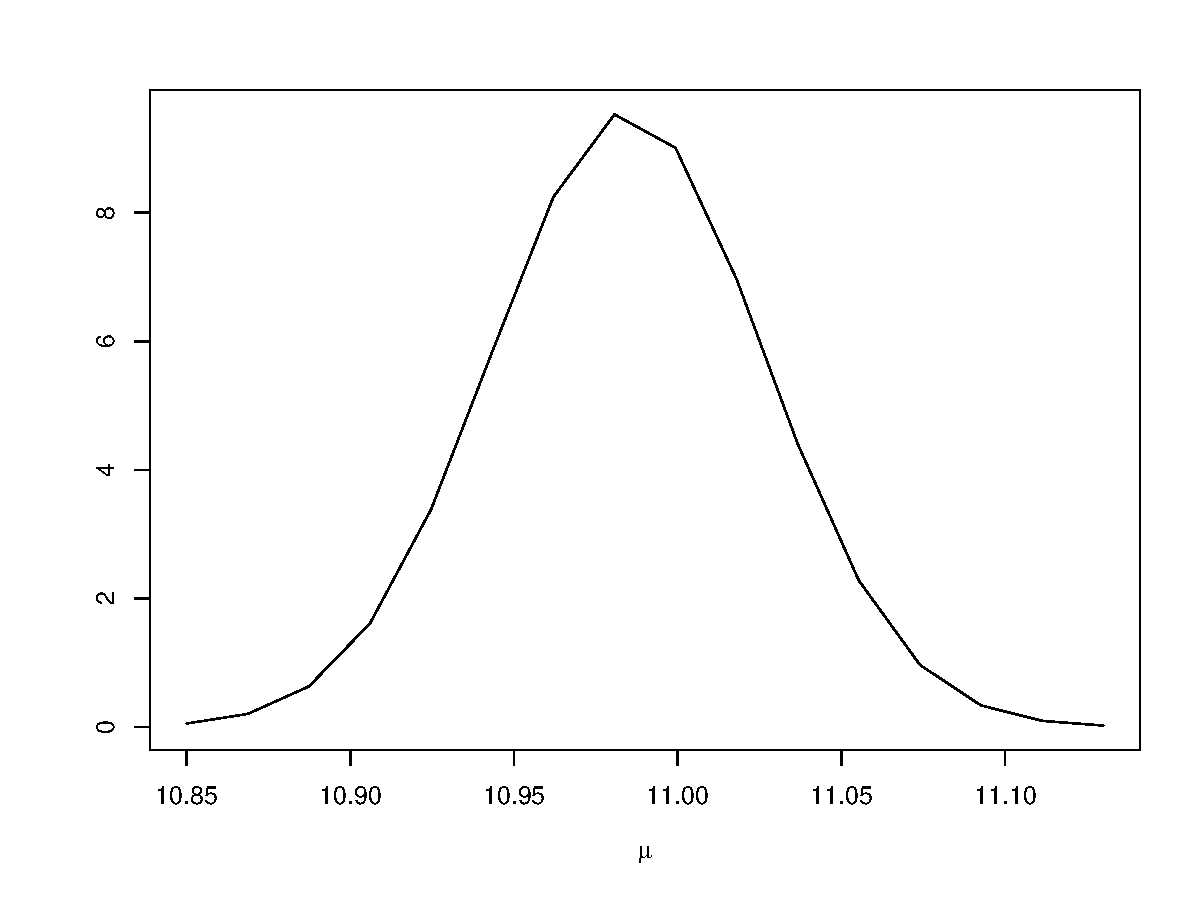
\includegraphics[scale=0.4]{figuras/dpm_mu_qr_15.pdf}}}%
	\qquad
	\subfloat[Densidade \textit{a posteriori} de $\sigma^2$]{{
			\label{fig:dpm_s2_qr_15}
			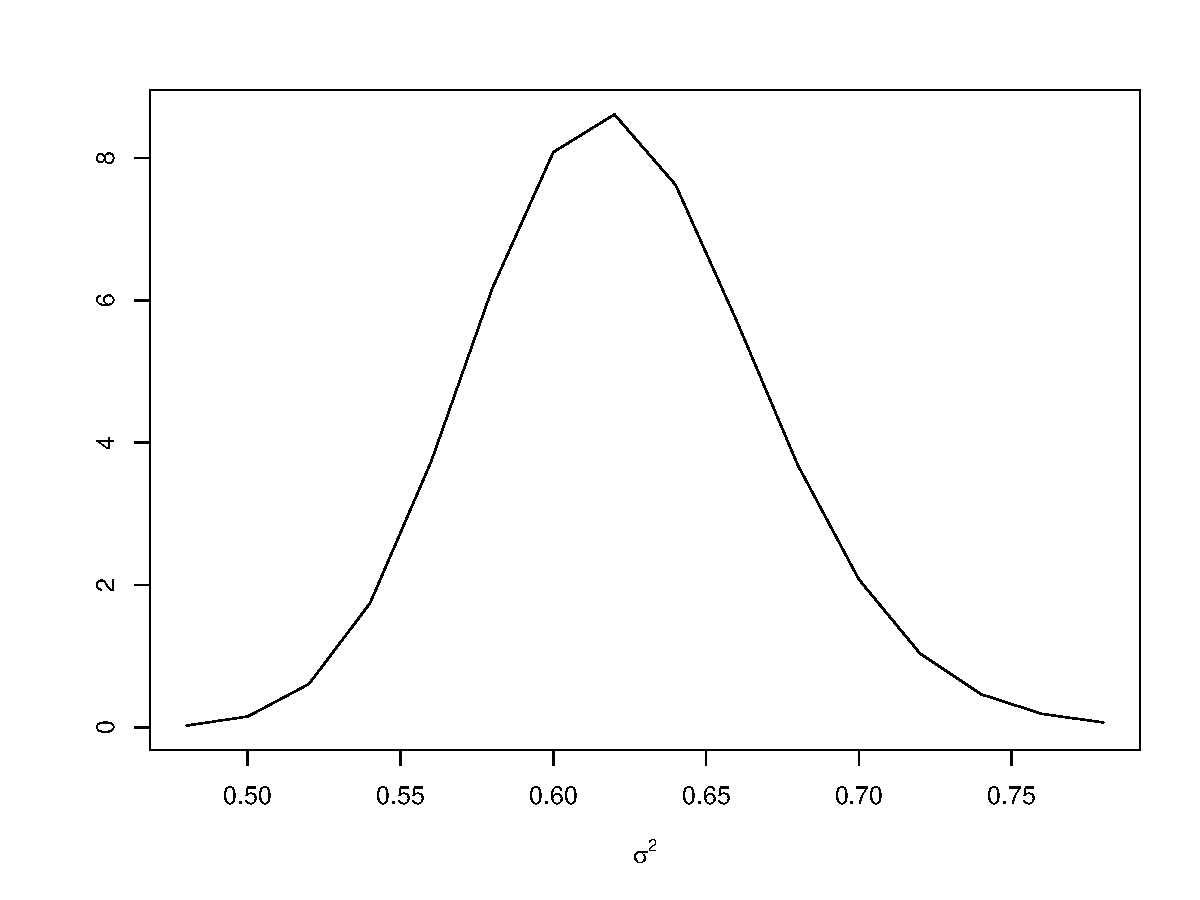
\includegraphics[scale=0.4]{figuras/dpm_s2_qr_15.pdf}}}%
	\subfloat[Densidade \textit{a posteriori} de $\nu$]{{
			\label{fig:dpm_nu_qr_15}
			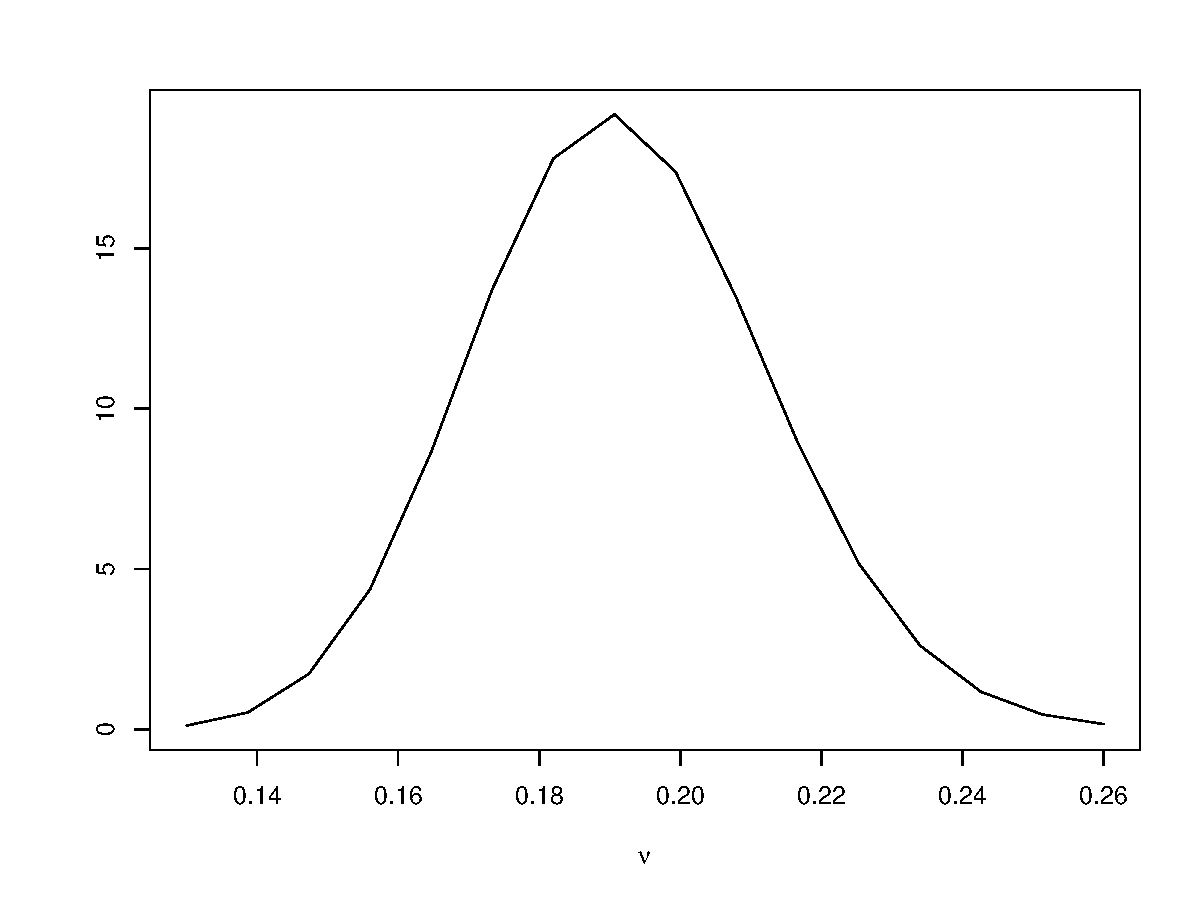
\includegraphics[scale=0.4]{figuras/dpm_nu_qr_15.pdf}}}%
	\caption{Densidades \textit{a posteriori} marginais pela quadratura de Riemann com $L = 15$}%
\end{figure}

\begin{figure}[t]%
	\centering
	\subfloat[Densidade \textit{a posteriori} de $\mu$]{{
			\label{fig:dpm_mu_qr_50}
			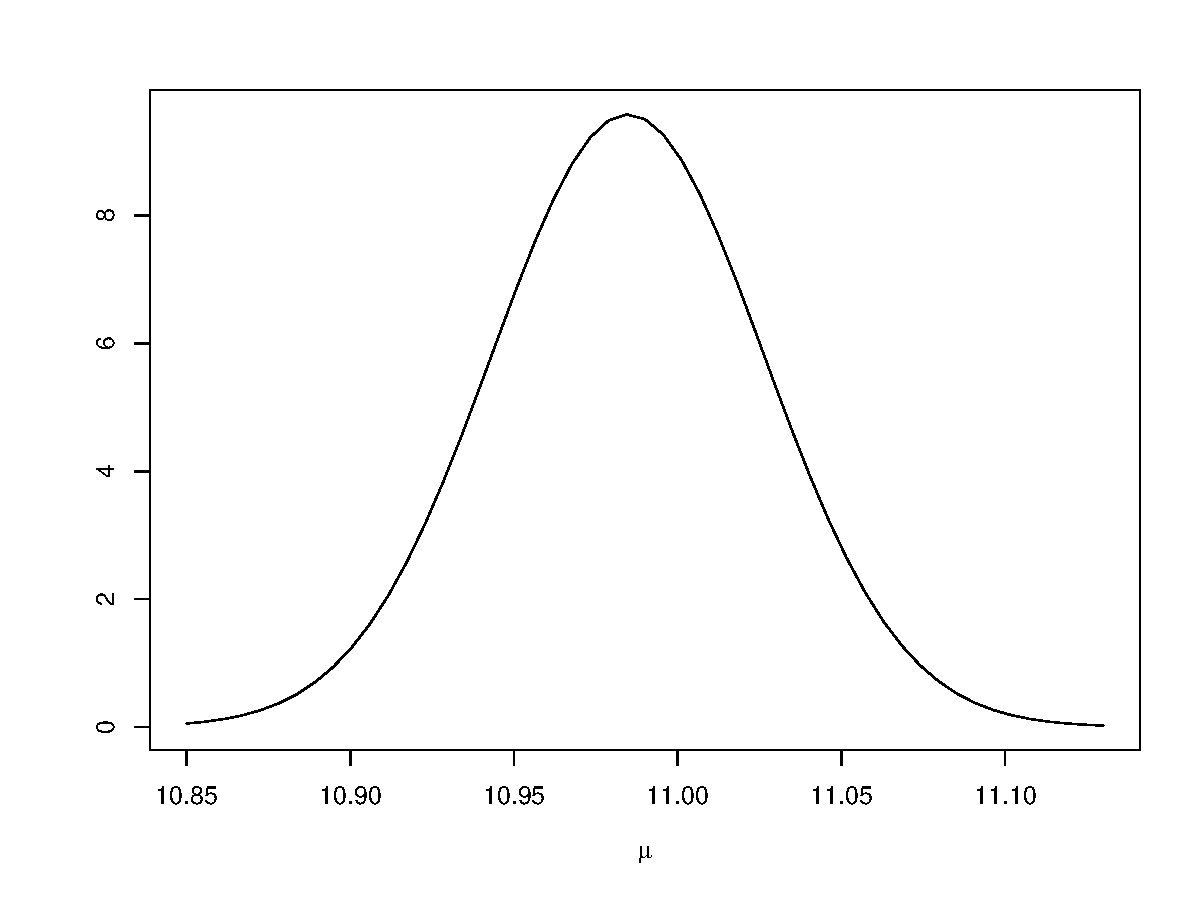
\includegraphics[scale=0.4]{figuras/dpm_mu_qr_50.pdf}}}%
	\qquad
	\subfloat[Densidade \textit{a posteriori} de $\sigma^2$]{{
			\label{fig:dpm_s2_qr_50}
			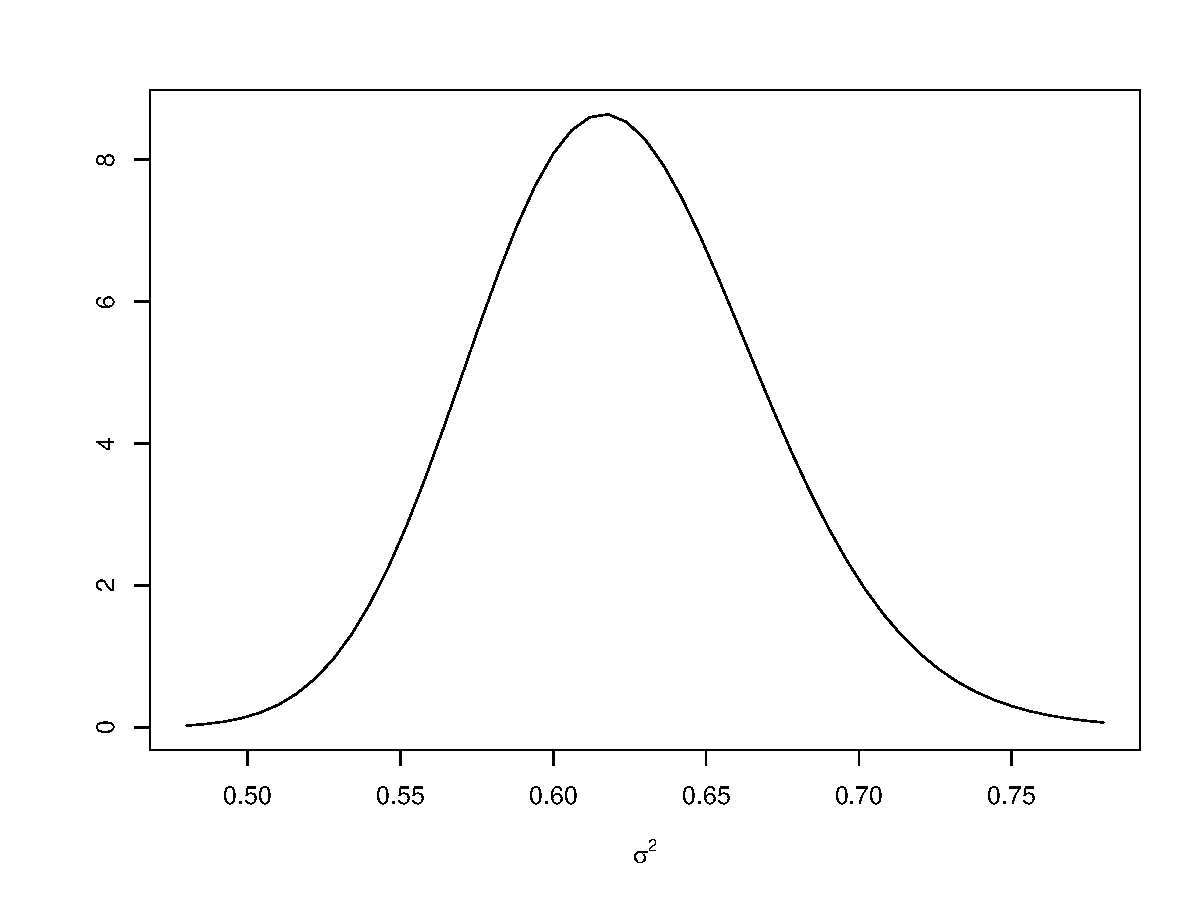
\includegraphics[scale=0.4]{figuras/dpm_s2_qr_50.pdf}}}%
	\subfloat[Densidade \textit{a posteriori} de $\nu$]{{
			\label{fig:dpm_nu_qr_50}
			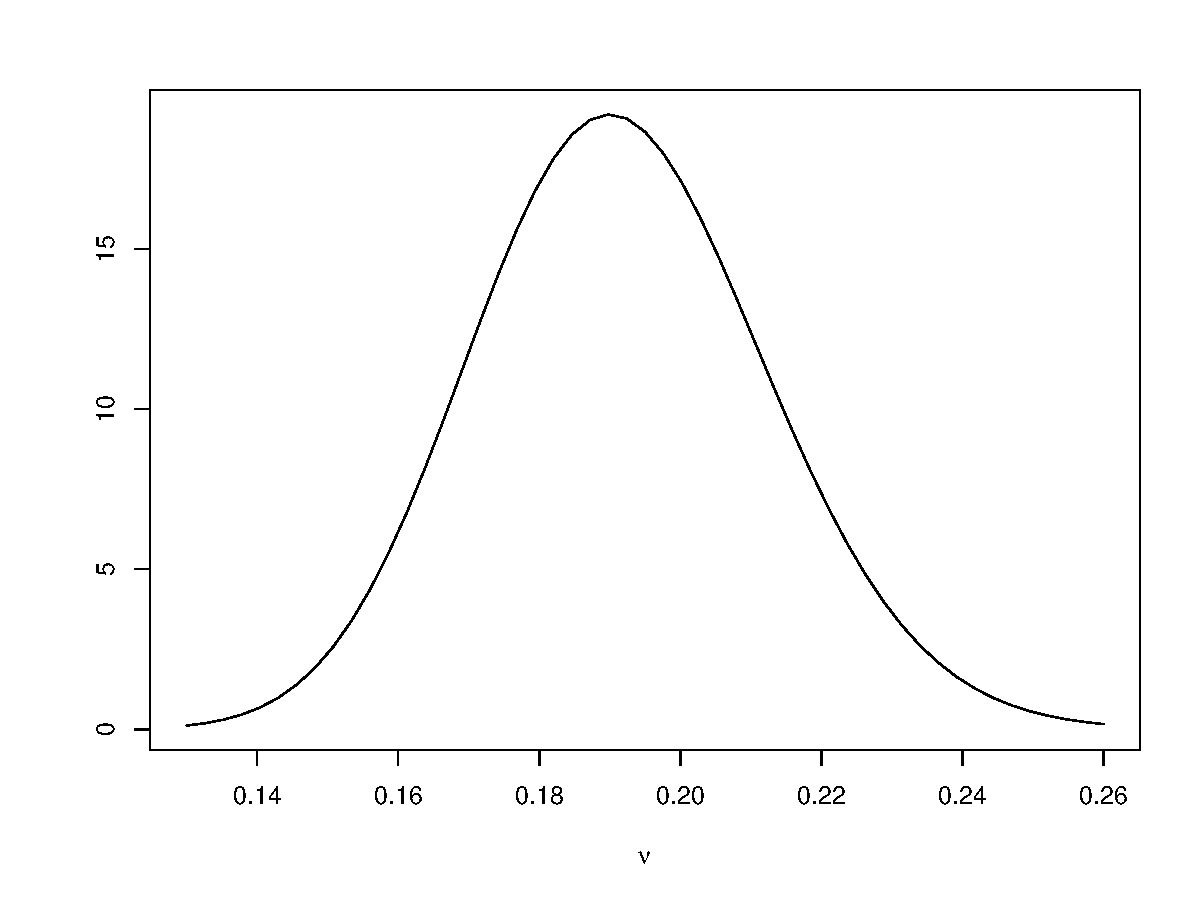
\includegraphics[scale=0.4]{figuras/dpm_nu_qr_50.pdf}}}%
	\caption{Densidades \textit{a posteriori} marginais pela quadratura de Riemann com $L = 50$}%
\end{figure}

\begin{figure}[t]%
	\centering
	\subfloat[Densidade \textit{a posteriori} de $\mu$]{{
			\label{fig:dpm_mu_qr_100}
			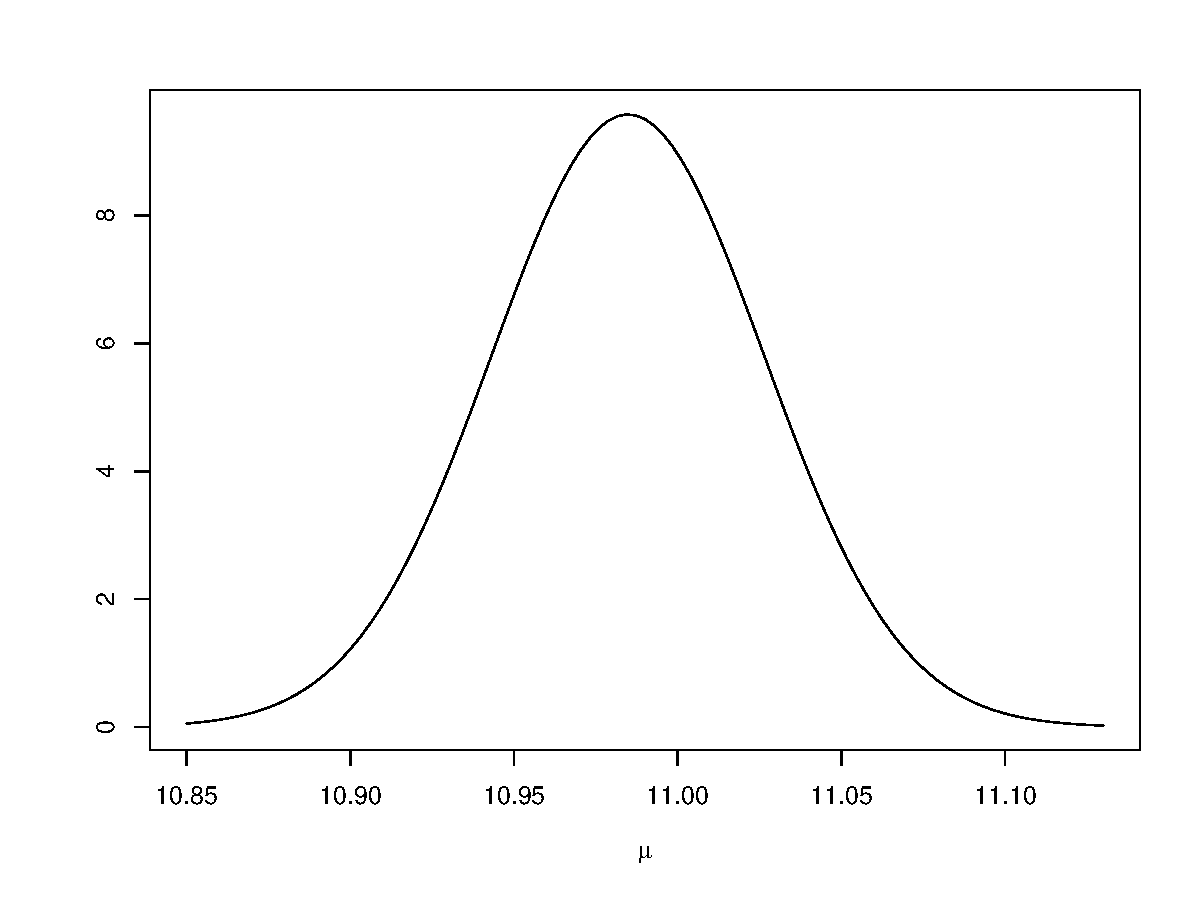
\includegraphics[scale=0.4]{figuras/dpm_mu_qr_100.pdf}}}%
	\qquad
	\subfloat[Densidade \textit{a posteriori} de $\sigma^2$]{{
			\label{fig:dpm_s2_qr_100}
			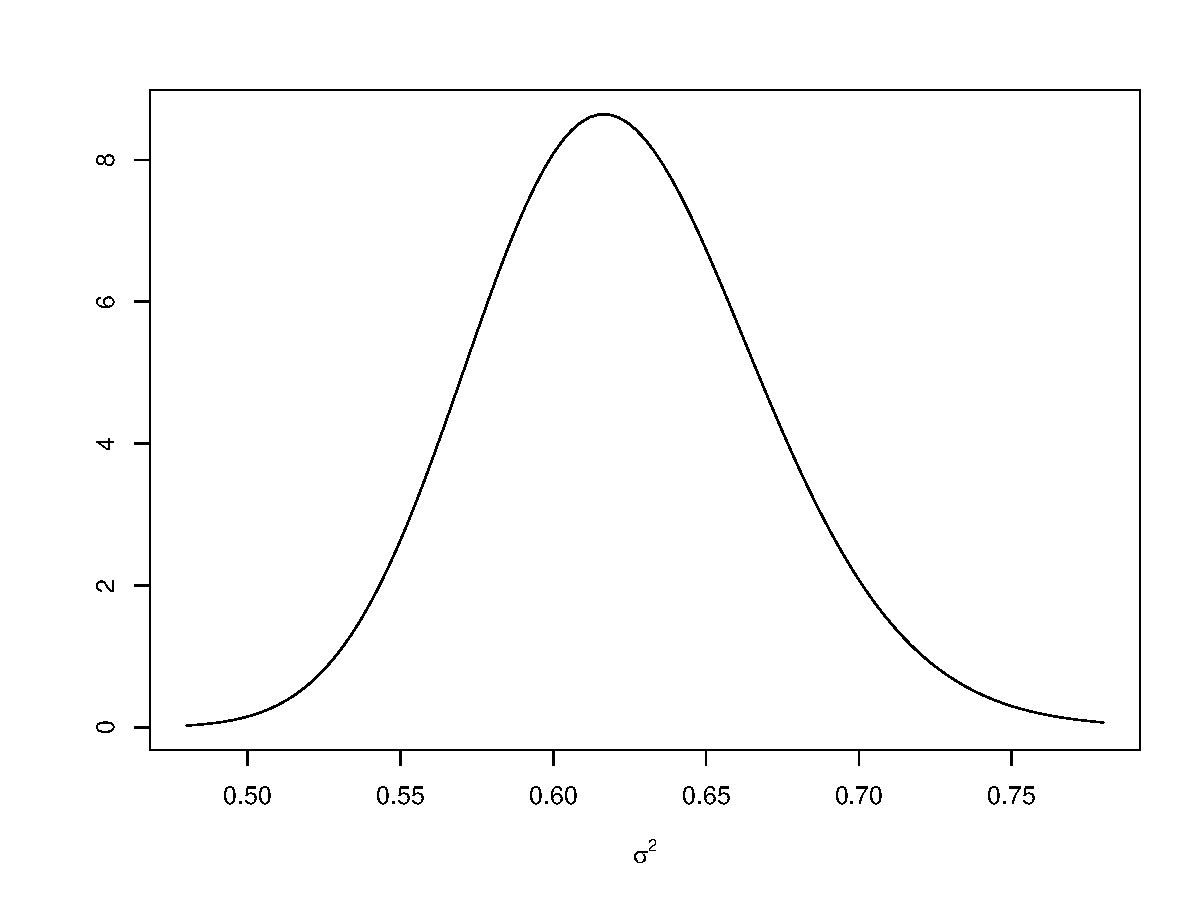
\includegraphics[scale=0.4]{figuras/dpm_s2_qr_100.pdf}}}%
	\subfloat[Densidade \textit{a posteriori} de $\nu$]{{
			\label{fig:dpm_nu_qr_100}
			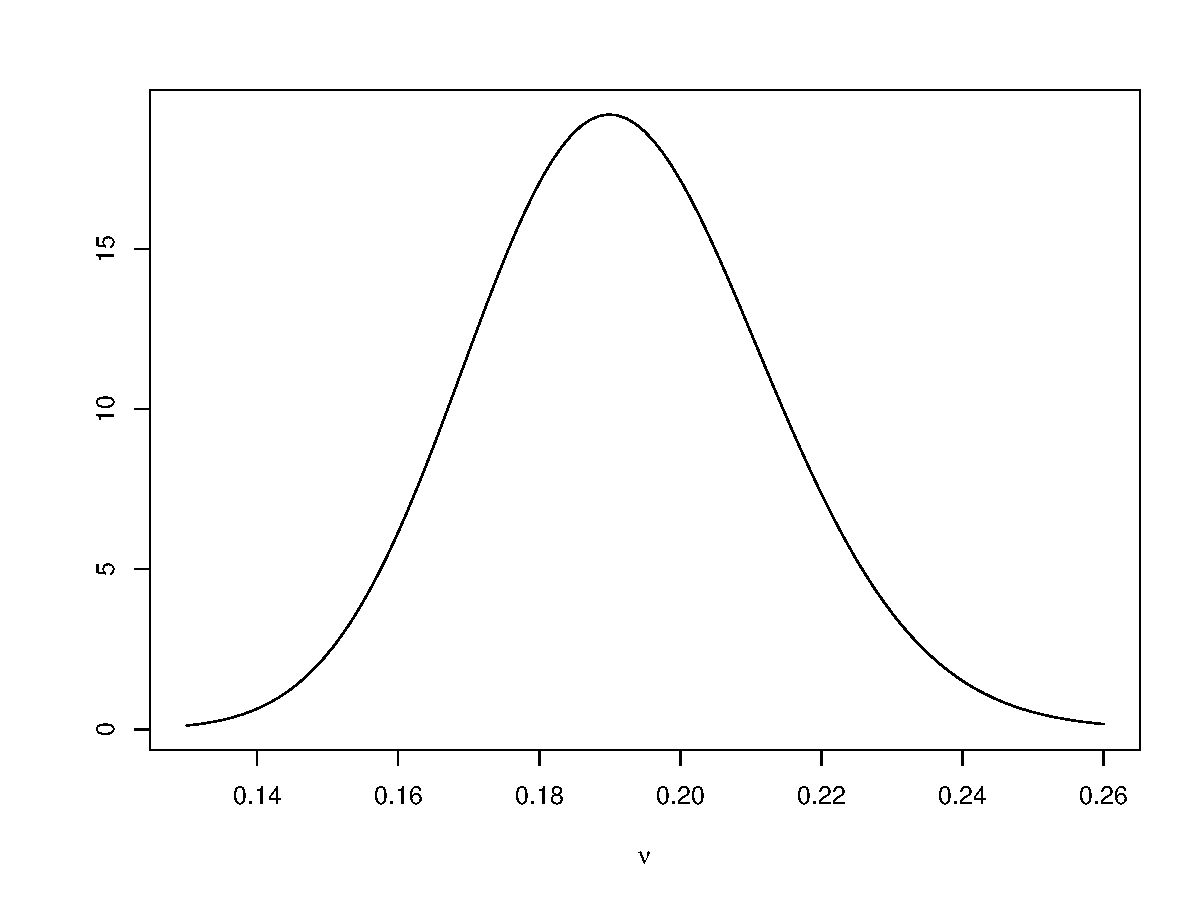
\includegraphics[scale=0.4]{figuras/dpm_nu_qr_100.pdf}}}%
	\caption{Densidades \textit{a posteriori} marginais pela quadratura de Riemann com $L = 100$}%
\end{figure}

Para $L=15$, a aproximação não é muito suave, mas começa a indicar como cada parâmetro se comporta com relação à locação e à dispersão de sua densidade \textit{a posteriori} marginal. Entretanto, ainda não é possível dizer como é o comportamento com relação à simetria.

Para $L=50$, a aproximação é bem suave. Além do comportamento com relação à locação e à dispersão, é possível dizer também como é o comportamento com relação à simetria da densidade \textit{a posteriori} marginal de cada parâmetro. Aparentemente, as densidades para $\sigma^2$ e $\nu$ são fracamente assimétricas à direita.

Para $L=100$, os gráficos confirma a tendência apresentada pelos dois cenários anteriores, mas com uma suavização ainda melhor. Porém, computacionalmente a integração numérica é bem mais demorada, uma vez que o número de pontos para cálculo das densidades \textit{a posteriori} marginais cresce a um fator de ordem $\mathcal{O}(L^3)$.

Obtidas as densidades \textit{a posteriori} marginais, é possível ainda estimar pela quadratura de Riemann os momentos \textit{a posteriori} de ordem $m$ para cada parâmetro e com os mesmos aproximar as estatísticas de média, variância, assimetria e curtose. Sem perda de generalidade, suponha que se deseja obter as estatísticas \textit{a posteriori} para $\alpha_1$. A aproximação pela quadratura de Riemann para um momento $m$ é dada por
\begin{align}
\mathbb{E}(\alpha_1^m | \bm{y}) &= \iint \alpha_1^m p(\alpha_1, \alpha_2, \alpha_3 | \bm{y}) d\alpha_1 d\alpha_2 d\alpha_3 \approx \sum_{i=1}^{L} \sum_{j=1}^{L} \sum_{k=1}^{L} r_i^m p(r_i, s_j, t_k | \bm{y}) \Delta_i \Delta_j \Delta_k \nonumber \\
&= \sum_{i=1}^{L} r_i^m \Delta_i \left[\sum_{j=1}^{L} \sum_{k=1}^{L} p(r_i, s_j, t_k | \bm{y}) \Delta_j \Delta_k\right] \nonumber \\
&= \sum_{i=1}^{L} r_i^m \Delta_i p(r_i | \bm{y}). \label{eq:mom_qr}
\end{align}

Como todas as estatísticas de interesse são funções dos quatro primeiros momentos, basta substituir $m = \{1, 2, 3, 4\}$ em \eqref{eq:mom_qr} para obter as respectivas aproximações. Na Tabela \ref{tab1}, são apresentados os valores aproximados para tais estatísticas em cada um dos três cenários.

\begin{table}[htb]
	\caption{Estatísticas \textit{a posteriori} para $(\mu, \sigma^2, \nu)$ pela quadratura de Riemann}
	\label{tab1}
	\centering
	\begin{tabular}{cccccc}
		\toprule
		Cenário & Parâmetro & Média & Variância & Assimetria & Curtose \\
		\midrule
		$L = 15$ & $\mu$      & 10.9847 & 0.0017 & 0.0022 & 2.9603 \\
				 & $\sigma^2$ &  0.6222 & 0.0022 & 0.2230 & 2.9984 \\
				 & $\nu$      &  0.1918 & 0.0004 & 0.1572 & 2.9348 \\
		\midrule
		$L = 50$ & $\mu$      & 10.9848 & 0.0017 & 0.0056 & 2.9346 \\
		         & $\sigma^2$ &  0.6222 & 0.0021 & 0.2149 & 2.9625 \\
		         & $\nu$      &  0.1918 & 0.0004 & 0.1523 & 2.8995 \\
		\midrule
		$L = 100$ & $\mu$      & 10.9848 & 0.0017 & 0.0064 & 2.9284 \\
		          & $\sigma^2$ &  0.6222 & 0.0021 & 0.2131 & 2.9542 \\
		          & $\nu$      &  0.1918 & 0.0004 & 0.1512 & 2.8913 \\
		\bottomrule
	\end{tabular}
\end{table}

Pela Tabela \ref{tab1}, pode-se concluir que tanto a média quanto a variância \textit{a posteriori} praticamente não variaram nos três cenários, independente do parâmetro considerado. Isto quer dizer que poucos subintervalos são necessários para se obter uma boa aproximação destas duas estatísticas. Por outro lado, o mesmo não pode ser dito para a assimetria e a curtose \textit{a posteriori}, para as quais há mudanças na terceira ou mesmo na segunda casa decimal, inclusive quando se passa de $L = 50$ para $L = 100$ subintervalos. Isto se explica pelo fato de que tanto a assimetria quanto a curtose são funções que dependem de vários momentos, até a terceira e quarta ordem respectivamente. Portanto, há maior dificuldade em aproximá-las. Apesar deste fato, para o problema considerado se pode dizer que houve uma estabilidade nas aproximações destas duas últimas estatísticas na medida em que a quantidade de subintervalos crescia.

Com relação aos valores em si, as médias \textit{a posteriori} para os 3 parâmetros ficaram bem próximas, mas não necessariamente iguais, aos respectivos valores do modelo para a distribuição amostral, mesmo para uma amostra muito grande ($n = 500$). É interessante notar que isso ocorre mesmo para o parâmetro $\nu$, cuja distribuição \textit{a priori} é não-informativa no sentido de Bayes-Laplace. Apesar disto, sua distribuição \textit{a posteriori} é influenciada pelas informações de $\mu$ e $\sigma^2$ contidas tanto nas distribuições \textit{a priori} correspondentes quanto na função de verossimilhança. Essa diferença já era esperada, uma vez que a aproximação é feita para a distribuição \textit{a posteriori} e não para a distribuição amostral.

Para as variâncias \textit{a posteriori}, todas elas foram bem pequenas, em especial para $\nu$. Isto se deve ao fato de que a amostra inicial dos dados era grande, portanto se poderia esperar uma redução na dispersão de cada parâmetro quando sua informação é atualizada com a distribuição amostral, por menos informativa que fosse a distribuição \textit{a priori} (como no caso de $\nu$). Com relação à assimetria \textit{a posteriori}, esta foi praticamente nula para $\mu$ e positiva, mas fraca, para $\sigma^2$ e $\nu$ (um pouco mais forte para a primeira). Por fim, as aproximações para a curtose \textit{a posteriori} foram todas bem próximas de 3, o valor encontrado para uma distribuição normal, com o parâmetro $\sigma^2$ mais próximo desse valor e $\nu$ o mais afastado.
\section{Reamostragem Por Importância Sequencial (SIR)}\label{sir}

Como uma das aproximações estocásticas a serem consideradas, o método da reamostragem por importância sequencial (SIR), ou reamostragem ponderada, foi uma das primeiras alternativas aos métodos de aproximação determinísticos previamente existentes. Se antes a densidade conjunta era aproximada por uma regra de quadratura, nas aproximações estocásticas o objetivo é simular amostras de uma densidade que aproxime a desejada com o menor erro possível. Este erro dependerá de $k$, o tamanho de uma amostra retirada da densidade aproximada, de ordem $\mathcal{O}(k^{-1})$, e não mais do conjunto de dados amostrais do modelo inicial.

Proposto por Gordon \textit{et al.} (1993)\cite{Gordon1993}, o método SIR utiliza uma \textit{função de amostragem por importância} $g$ para aproximar (sem perda de generalidade) uma densidade de interesse $p$. Neste caso, $g$ é uma densidade conhecida e da qual se sabe gerar uma amostra aleatória. Cada ponto selecionado na amostra de $g$ é ponderado para corrigir a probabilidade de amostragem de tal forma que a amostra ponderada aproxime uma outra que seria extraída da densidade de $p$ caso se soubesse gerar da mesma. Os pesos usados para corrigir as probabilidades de amostragem são chamados \textit{pesos de importância padronizados}. Sejam $\theta_1, \ldots, \theta_k$ uma amostra aleatória de $g$ e $\bm{y} = (y_1, \ldots, y_n)$ uma amostra do modelo para os dados observados. Para cada ponto $\theta_j$, $j = 1, \ldots, k$, os pesos são dados por
\begin{equation}\label{eq:sir_wei}
w_j(\theta_j) = \dfrac{p(\theta_j | \bm{y}) / q(\theta_j)}{\sum_{j=1}^{k} p(\theta_j | \bm{y}) / q(\theta_j)}.
\end{equation}

Após gerar cada valor $w_j(\theta_j)$, uma reamostragem é feita do suporte discreto $\theta_1, \ldots, \theta_k$ com probabilidades $w_1(\theta_1), \ldots, w_k(\theta_k)$. A nova amostra resultante terá uma distribuição aproximadamente igual à de $p$, convergindo para esta quando $k \rightarrow \infty$. Em outras palavras, diz-se que o método SIR gera uma amostra de $p$ assintoticamente. Observe que a densidade $g$ a ser escolhida deve ter o mesmo suporte de $p$ para que o método funcione.

No presente trabalho, tem-se 3 parâmetros ($\mu, \sigma^2$ e $\nu$) a serem gerados dada uma densidade \textit{a posteriori} $p(\mu, \sigma^2, \nu | \bm{x})$. Como esta densidade possui uma constante de proporcionalidade $c$ associada, pela razão do lado direito de \eqref{eq:sir_wei} esta é cancelada, sendo possível trabalhar apenas com o núcleo de $p(\mu, \sigma^2, \nu | \bm{x})$ calculado no lado direito em \eqref{eq:dist_post}. Isto por si só é uma vantagem do método SIR em relação à quadratura de Riemann, para a qual se viu que era necessário aproximar $c$. Como se deseja aproximar uma função conjunta de 3 parâmetros, a densidade $g$ a ser escolhida deve não apenas ter a mesma dimensão, mas também cada uma de suas componentes marginais deve ter o mesmo suporte do parâmetro correspondente no núcleo de $p(\mu, \sigma^2, \nu | \bm{x})$.

Como feito em muitos trabalhos, para $g$ será escolhida uma densidade normal trivariada $N_3(\bm{\mu}, \bm{\Sigma})$, cujas componentes têm, cada uma, suporte em toda a reta real. Note que para 2 parâmetros, $\sigma^2$ e $\nu$, o respectivo espaço paramétrico não é a reta real ($\Theta_{\sigma^2} = \mathbb{R}_+$ e $\Theta_{\nu} = [0,1]$, respectivamente). Desta forma, antes de usar o método é necessário reparametrizar \eqref{eq:dist_post} de modo que todos os novos parâmetros tenham suporte em $\mathcal{R}$. Para a reparametrização, consideram-se as transformações $\theta_1 = \mu, \theta_2 = \log(\sigma^2)$ e $\theta_3 = \log[\nu/(1-\nu)]$. Logo, a expressão do núcleo reparametrizado é dada por
\begin{align}
p(\theta_1, \theta_2, \theta_3 | \bm{x})
&= p(\theta_1 = \mu, \theta_2 = \log(\sigma^2), \theta_3 = \log[\nu/(1-\nu)] | \bm{x}) \nonumber \\
&= p(\mu = \theta_1, \sigma^2 = \exp(\theta_2), \nu = 1/[1 + \exp(-\theta_3)] | \bm{x}) \times |J(\theta_1, \theta_2, \theta_3)| \nonumber \\
&\propto \left[\exp(\theta_2)\right]^{-[(n + 1)/2 + a + 1]} \times \exp\left\{-\dfrac{\left[(\theta_1 - m)^2 / (2V) + d\right]}{\exp(\theta_2)}\right\} \nonumber \\
&\times A^*(\bm{x} | \theta_1, \theta_2, \theta_3) \times  \dfrac{\exp(\theta_2) \exp(\theta_3)}{\left[1 + \exp(-\theta_3)\right]^{-2}} \nonumber \\
&\propto \left(\dfrac{1}{\sigma^2}\right)^{(n + 1)/2 + a + 1} \times \exp\left\{-\dfrac{\left[(\mu - m)^2 / (2V) + d\right]}{\sigma^2}\right\} \times A(\bm{x} | \mu, \sigma^2, \nu) \nonumber \\
&\times \sigma^2 \nu^3(1-\nu)^{-1}, \label{eq:sir_dpre}
\end{align}
onde $|J(\theta_1, \theta_2, \theta_3)|$ é o determinante da matriz jacobiana das derivadas parciais de $(\mu, \sigma^2, \nu)$ com respeito a $(\theta_1, \theta_2, \theta_3)$. No cálculo deste determinante, todos os elementos fora da diagonal principal da matriz jacobiana serão nulos, já que na reparametrização utilizada não se assumiu nenhuma função dependente de mais de um parâmetro.

Novamente, para a versão reparametrizada do núcleo da densidade em \eqref{eq:sir_dpre} deve-se primeiro tomar o logaritmo de cada termo em seu produto para só depois exponenciá-la, de modo a evitar problemas numéricos. Para a amostra de tamanho $n=500$ da mistura finita de normais com variância contaminada tal que $\mu = 11$; $\sigma^2 = 0.64$; $\nu = 0.2$; $m = 11$; $V = 1$; $a = 7$ e $d = 4$ (Figura \ref{fig:sample_n.pdf}), o logaritmo do núcleo da densidade \textit{a posteriori} reparametrizada é igual a $-523.9575$ (bem próximo do valor na parametrização original), cuja exponencial é aproximadamente igual a $2.806 \times 10^{-228}$.

Os gráficos das densidades \textit{a posteriori} marginais para cada parâmetro quando os demais são fixados nos seus valores verdadeiros (Figuras \ref{fig:maspro_mu} a \ref{fig:maspro_nu}), os quais fornecem os respectivos intervalos de massa probabilística, novamente serão úteis, mas agora para definir a parametrização da distribuição normal trivariada a ser usada no método SIR. Para as médias das componentes desta distribuição, será fixado $\bm{\mu} = (\theta_1, \theta_2, \theta_3) = (\mu, \log(\sigma^2), \log[\nu/(1-\nu)]) = (11, \log(0.64), \log[0.2/0.8])$. Para a matriz de covariância $\bm{\Sigma}$, cada elemento da diagonal principal será dado pelo quadrado de $1/6$ do intervalo de massa probabilística do parâmetro correspondente. Esta escolha se justifica pelo fato de que as distribuições mostradas de \ref{fig:maspro_mu} a \ref{fig:maspro_nu} têm comportamento próximo à normalidade. Para uma distribuição normal, $99.7\%$ de sua massa probabilística está concentrada a até uma distância de 3 vezes o seu desvio padrão em relação ao ponto médio. Para os elementos fora da diagonal principal de $\bm{\Sigma}$, todos foram assumidos iguais a zero. Desta forma, $\bm{\Sigma} = \textrm{diag}\{0.0022, 0.0065, 0.0203\}$.

Escolhida a densidade $g$, resta aplicar o método SIR para obter amostras \textit{a posteriori} de $\mu$, $\sigma^2$ e $\nu$. Para este trabalho, foram considerados 3 cenários: $k = \{500, 5000, 50000\}$. Em cada cenário, foram geradas amostras de cada componente de $g$. Cada ponto amostral foi reparametrizado (quando fosse o caso) de volta para obter os valores estimados de $\mu$, $\sigma^2$ e $\nu$. Por fim, para todos os pontos amostrais de $g$ também foi calculado o valor da densidade conjunta, necessária para obter os pesos de importância padronizados do método SIR. Construído o suporte discreto para cada parâmetro a partir dos pontos amostrais da componente de $g$ correspondente, amostras \textit{a posteriori} são obtidas associando cada peso ao ponto amostral correspondente de $g$. Nas figuras \ref{fig:mu_sir_500} a \ref{fig:nu_sir_500}; \ref{fig:mu_sir_5000} a \ref{fig:nu_sir_5000} e \ref{fig:mu_sir_50000} a \ref{fig:nu_sir_50000} são apresentados os histogramas para as amostras \textit{a posteriori} de cada parâmetro por cenário.

\begin{figure}[t]%
	\centering
	\subfloat[Histograma de $\mu$]{{
			\label{fig:mu_sir_500}
			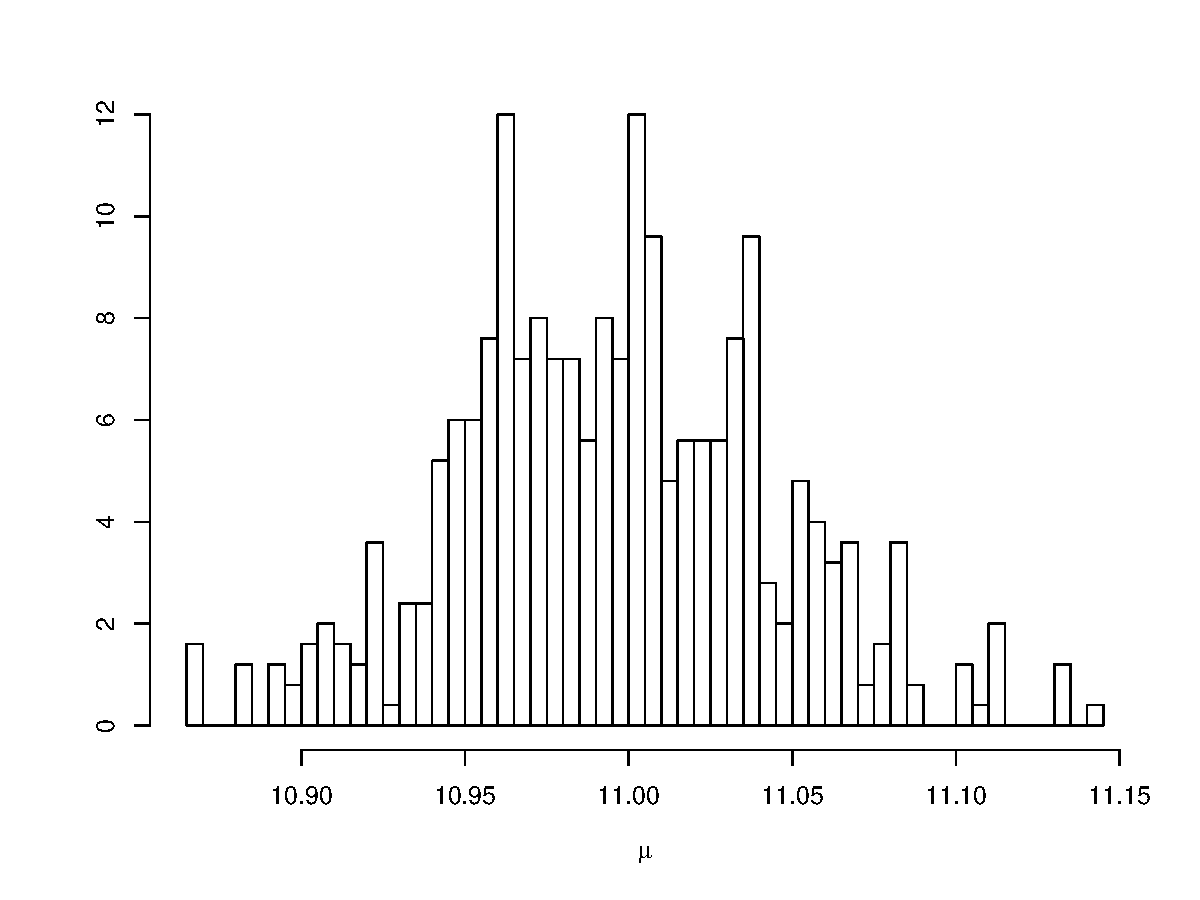
\includegraphics[scale=0.4]{figuras/mu_sir_500.pdf}}}%
	\qquad
	\subfloat[Histograma de $\sigma^2$]{{
			\label{fig:s2_sir_500}
			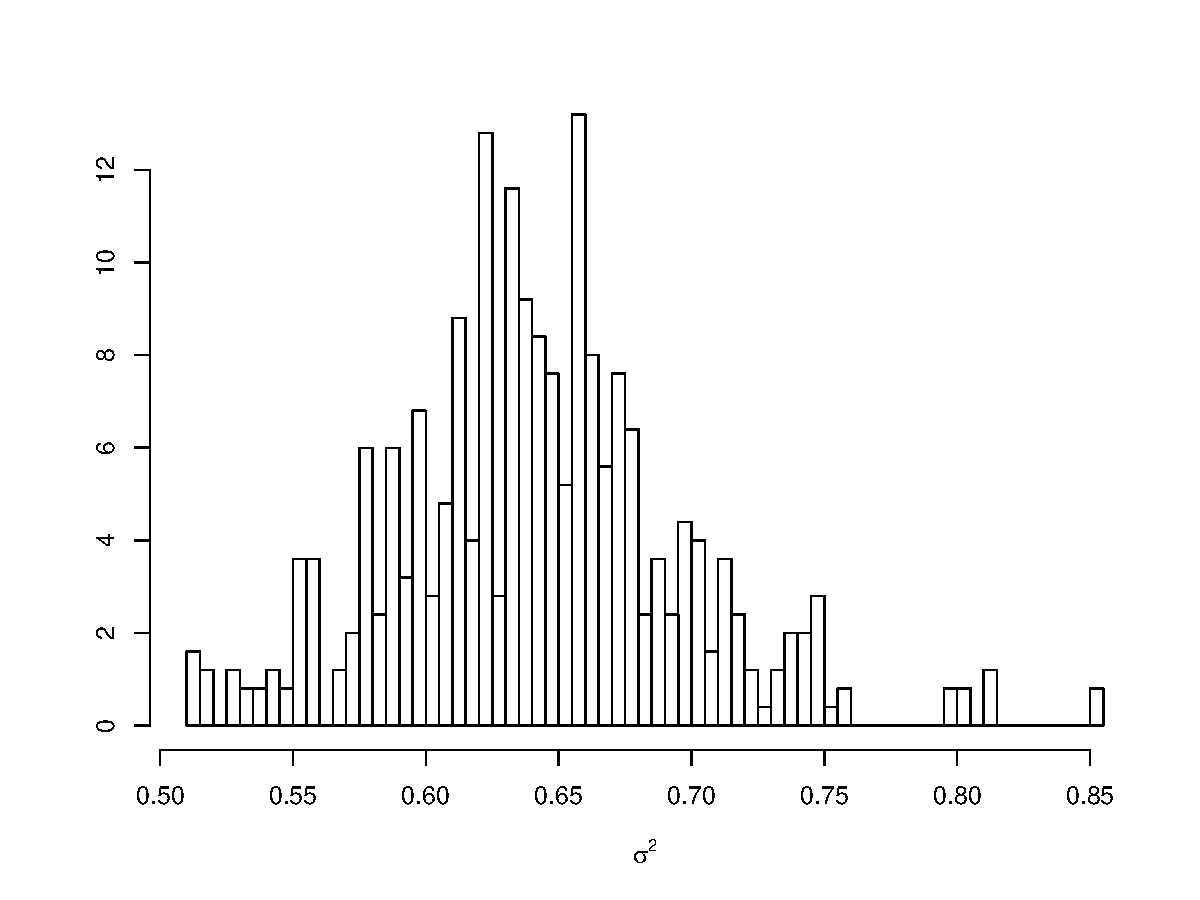
\includegraphics[scale=0.4]{figuras/s2_sir_500.pdf}}}%
	\subfloat[Histograma de $\nu$]{{
			\label{fig:nu_sir_500}
			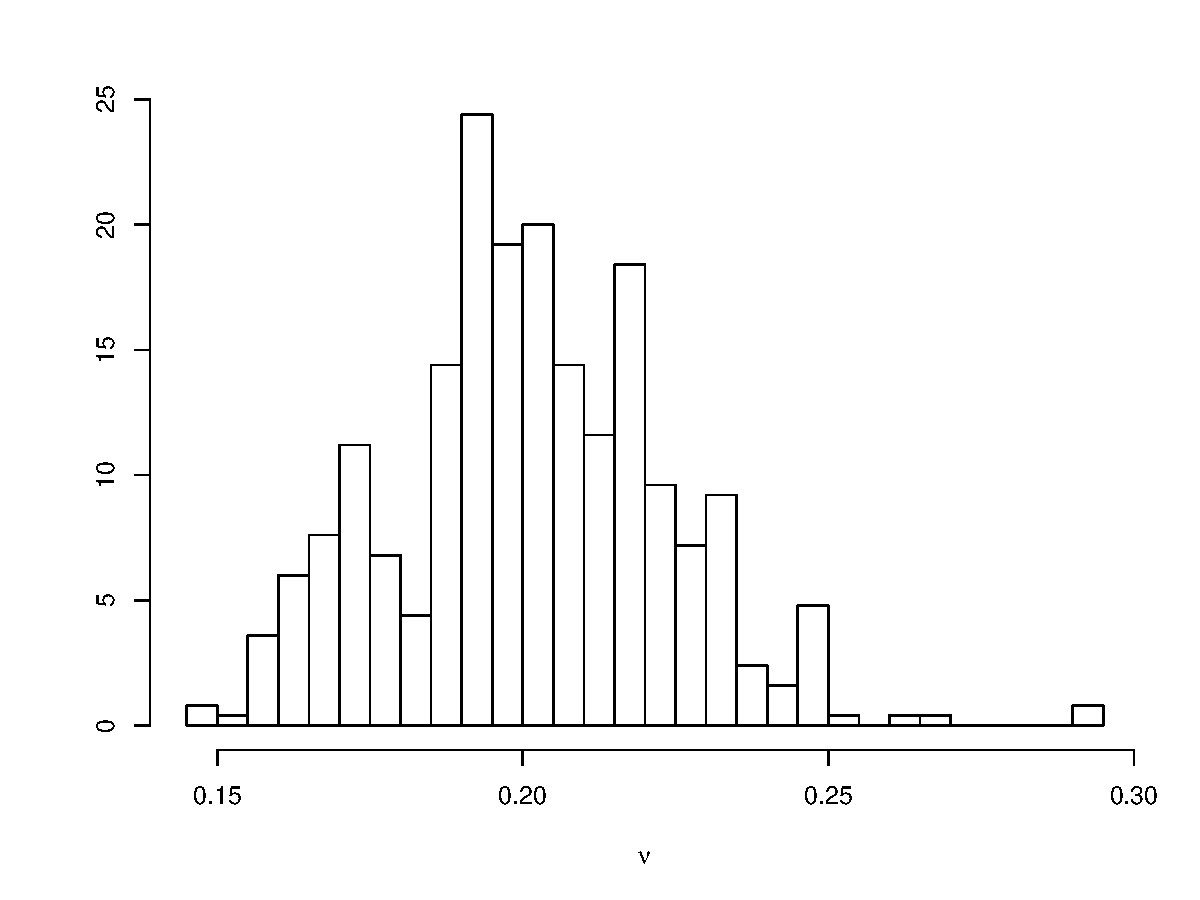
\includegraphics[scale=0.4]{figuras/nu_sir_500.pdf}}}%
	\caption{Histograma das densidades \textit{a posteriori} marginais pela método SIR com $k = 500$}%
\end{figure}

\begin{figure}[t]%
	\centering
	\subfloat[Histograma de $\mu$]{{
			\label{fig:mu_sir_5000}
			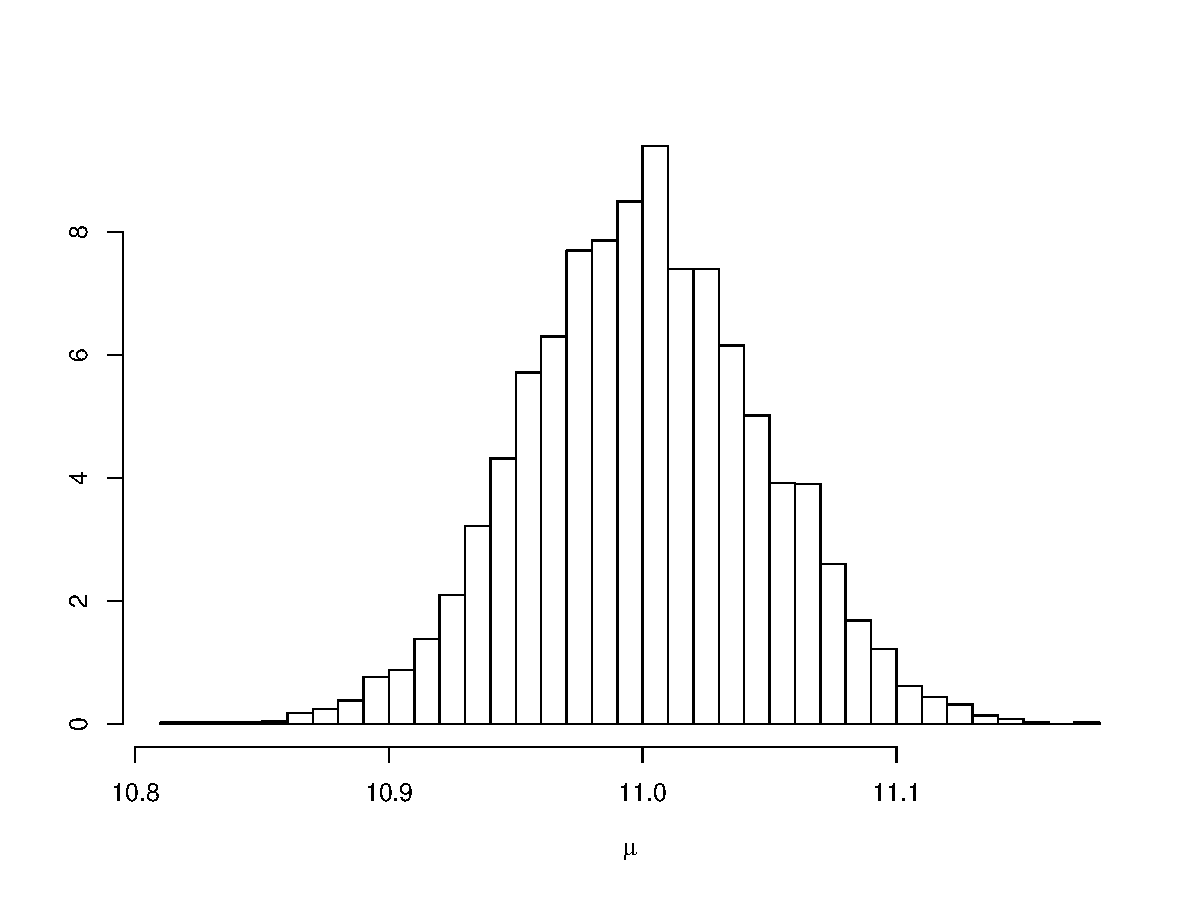
\includegraphics[scale=0.4]{figuras/mu_sir_5000.pdf}}}%
	\qquad
	\subfloat[Histograma de $\sigma^2$]{{
			\label{fig:s2_sir_5000}
			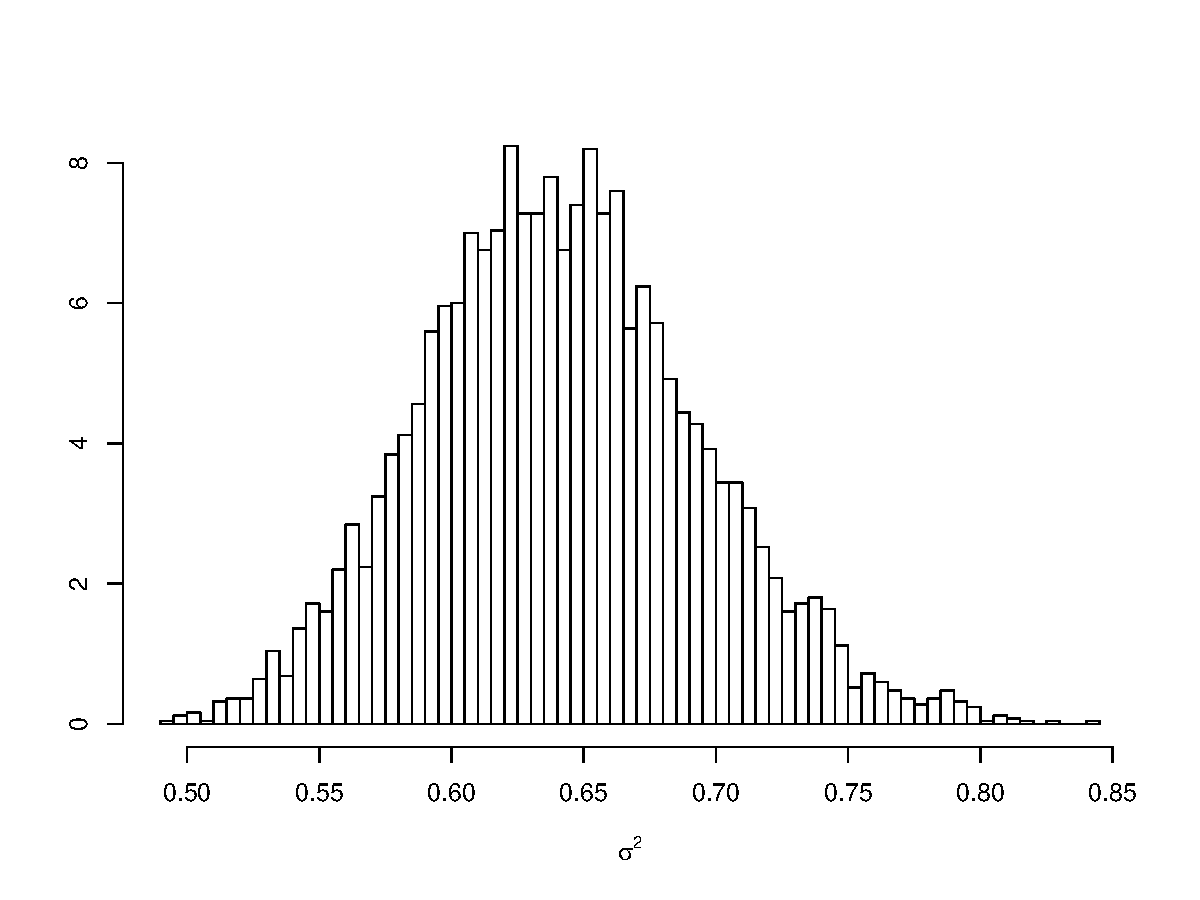
\includegraphics[scale=0.4]{figuras/s2_sir_5000.pdf}}}%
	\subfloat[Histograma de $\nu$]{{
			\label{fig:nu_sir_5000}
			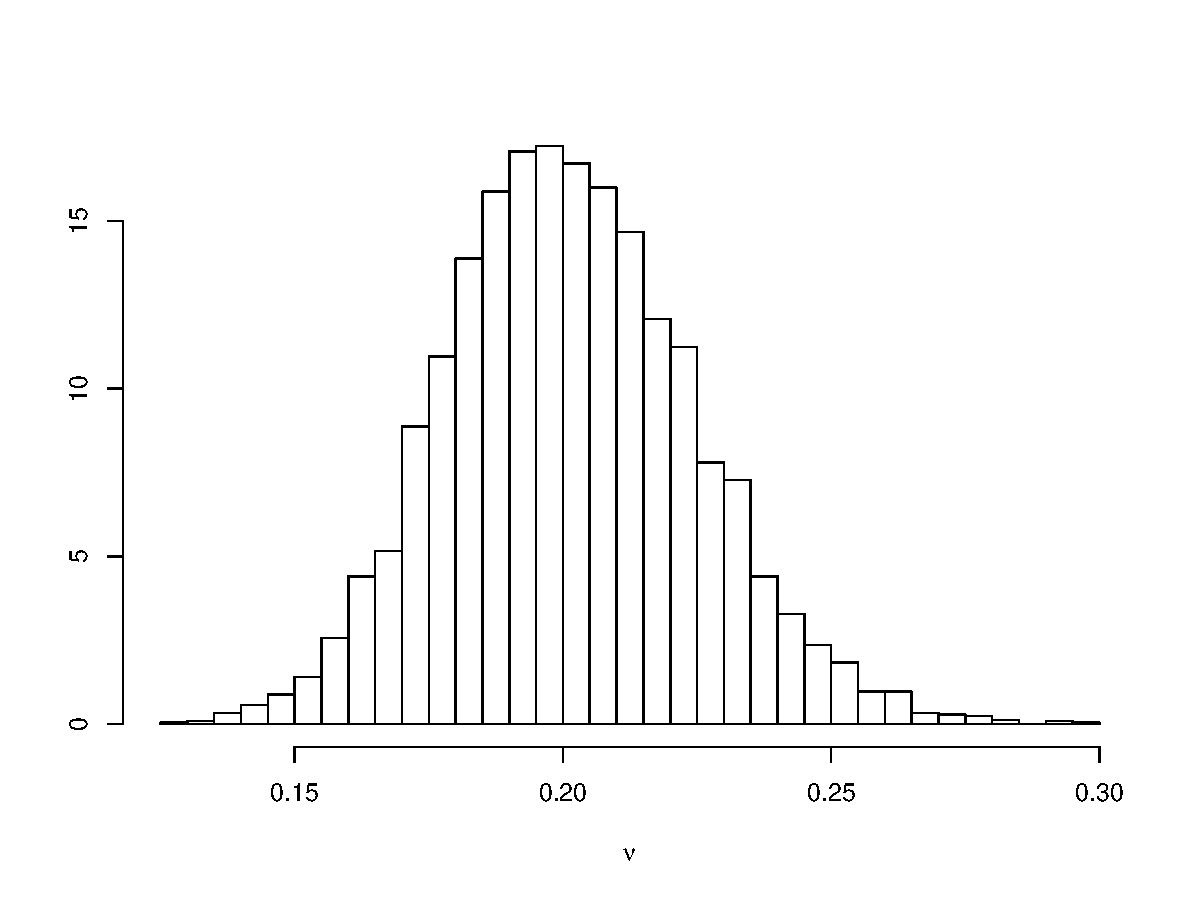
\includegraphics[scale=0.4]{figuras/nu_sir_5000.pdf}}}%
	\caption{Histograma das densidades \textit{a posteriori} marginais pela método SIR com $k = 5000$}%
\end{figure}

\begin{figure}[t]%
	\centering
	\subfloat[Histograma de $\mu$]{{
			\label{fig:mu_sir_50000}
			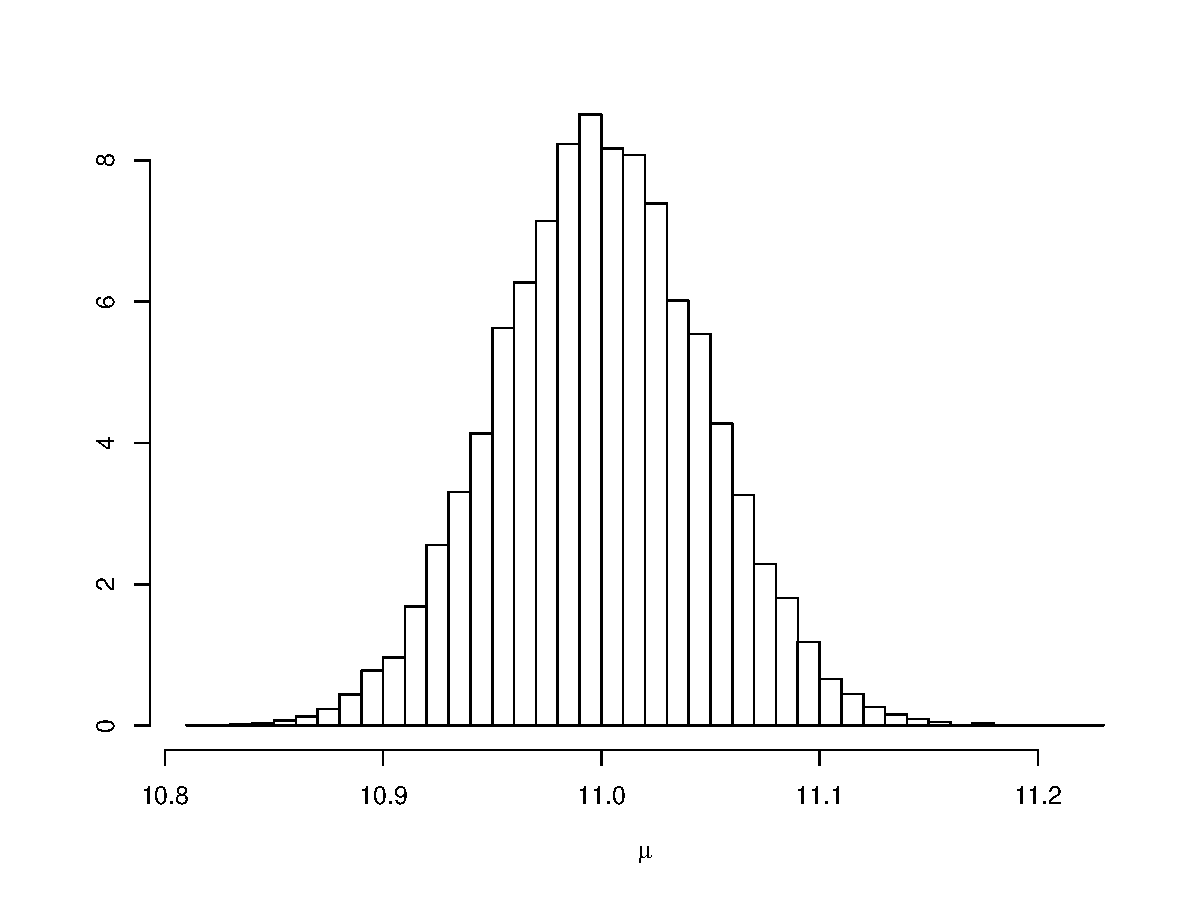
\includegraphics[scale=0.4]{figuras/mu_sir_50000.pdf}}}%
	\qquad
	\subfloat[Histograma de $\sigma^2$]{{
			\label{fig:s2_sir_50000}
			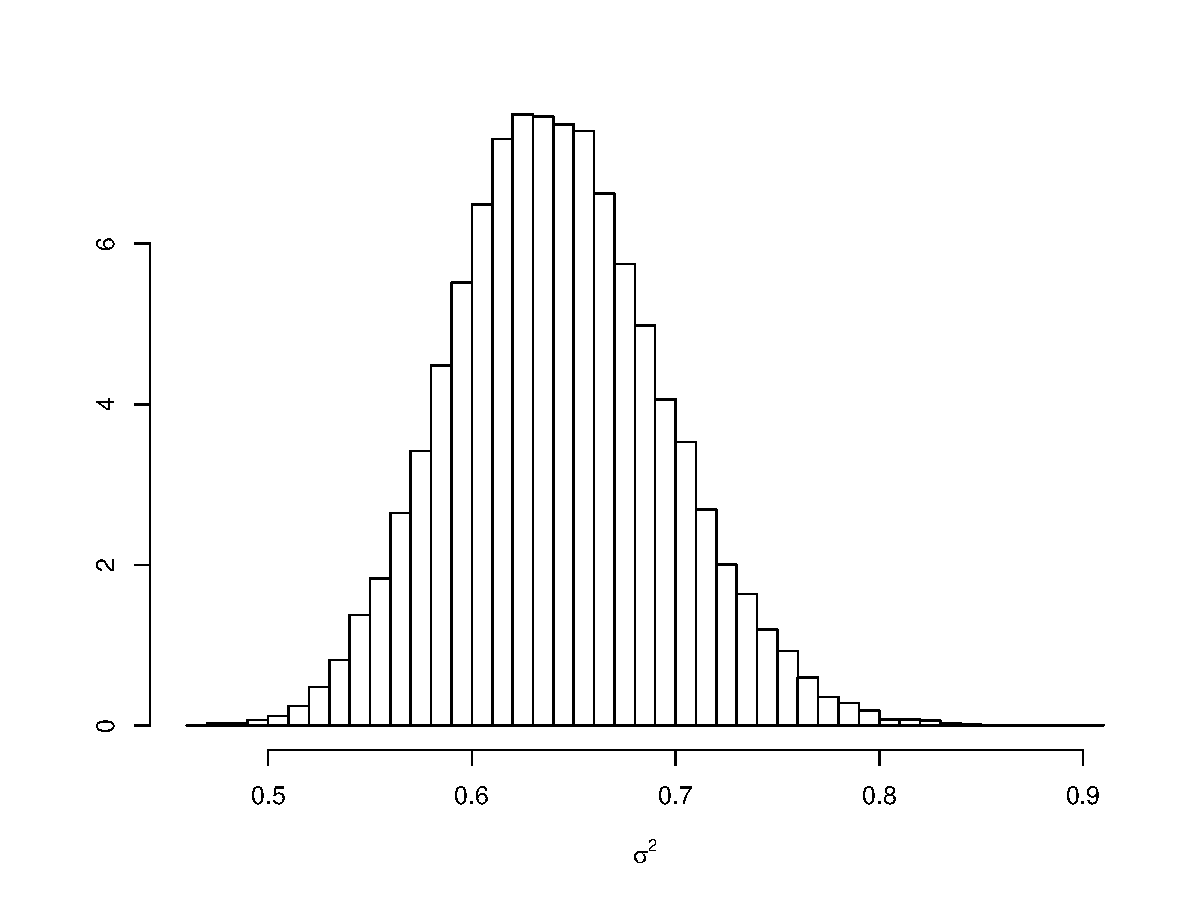
\includegraphics[scale=0.4]{figuras/s2_sir_50000.pdf}}}%
	\subfloat[Histograma de $\nu$]{{
			\label{fig:nu_sir_50000}
			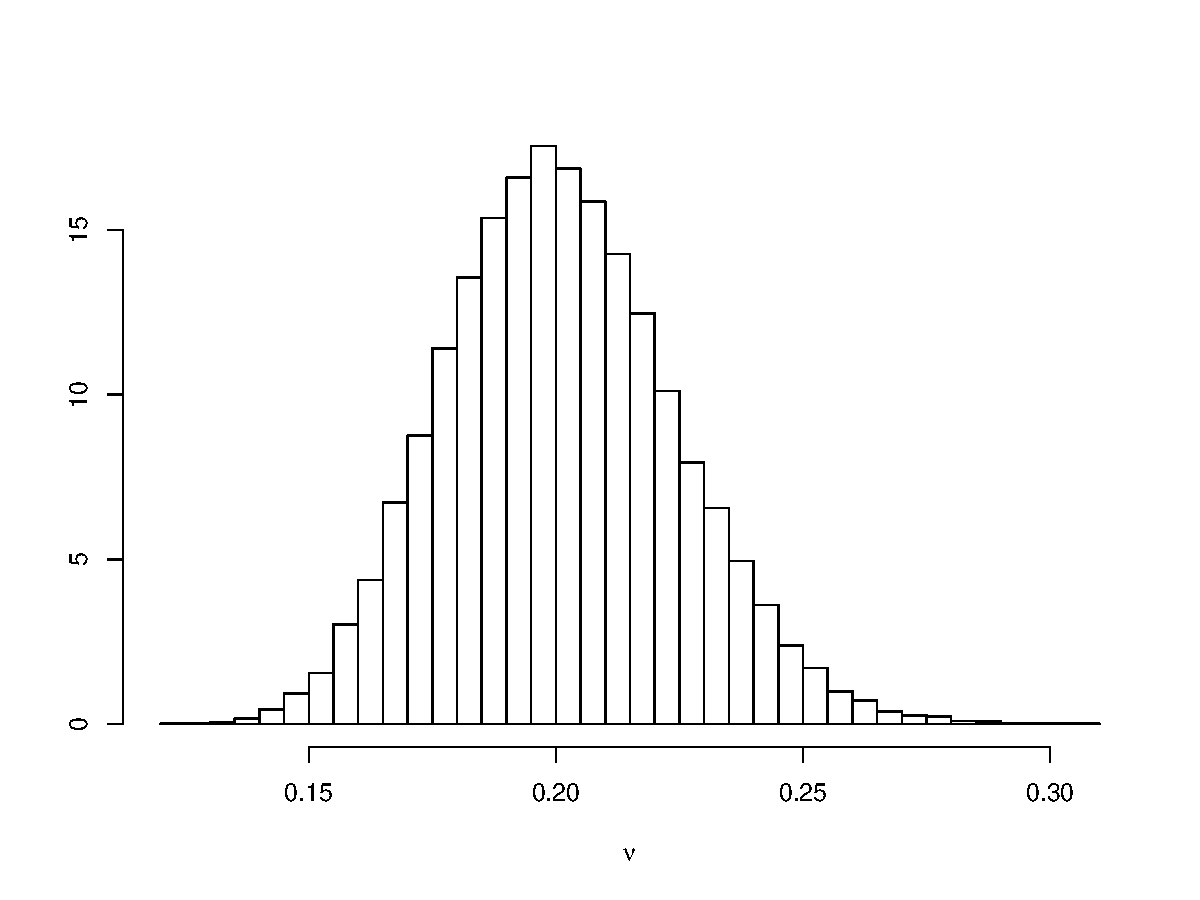
\includegraphics[scale=0.4]{figuras/nu_sir_50000.pdf}}}%
	\caption{Histograma das densidades \textit{a posteriori} marginais pela método SIR com $k = 50000$}%
\end{figure}

Para $k=500$, a aproximação da densidade não é boa para nenhum dos 3 parâmetros: há alguns pontos extremos (em inglês, \textit{outliers}) distantes do que seria a massa principal, especialmente para $\sigma^2$. Além disso, há vários pontos de máximo locais (modas), indicando uma curva longe de ser suave. Entretanto, é possível dizer já neste cenário como é o comportamento de cada parâmetro com relação à locação.

Para $k=5000$, a aproximação é muito mais suave e há bem menos \textit{outliers}. O número de modas locais também é severamente reduzido em comparação ao cenário anterior, embora esta quantidade ainda seja moderada para $\mu$. Além do comportamento com relação à locação, é possível dizer também como é o comportamento com relação à dispersão e à simetria da densidade \textit{a posteriori} marginal de cada parâmetro. Aparentemente, as densidades para $\sigma^2$ e $\nu$ são fracamente assimétricas à direita.

Para $k=50000$, os gráficos confirmam a tendência apresentada pelo cenário anterior, mas com uma suavização ainda melhor. Agora, todas as distribuições são unimodais e não há mais \textit{outliers}. Computacionalmente, a reamostragem é um pouco mais demorada, mas não na mesma taxa da quadratura de Riemann, já que agora o número de pontos amostrais cresce a um fator de ordem $\mathcal{O}(k)$, logo de modo linear.

Obtidas as amostras \textit{a posteriori} marginais de cada parâmetro, para aproximar as estatísticas de média, variância, assimetria e curtose é suficiente que se tomem as respectivas estimativas amostrais. Na Tabela \ref{tab2}, são apresentados os valores aproximados para tais estatísticas em cada um dos três cenários.

\begin{table}[htb]
	\caption{Estatísticas \textit{a posteriori} para $(\mu, \sigma^2, \nu)$ pelo método SIR}
	\label{tab2}
	\centering
	\begin{tabular}{cccccc}
		\toprule
		Cenário & Parâmetro & Média & Variância & Assimetria & Curtose \\
		\midrule
		$k = 500$ & $\mu$      & 10.9956 & 0.0024 & 0.1394 & 3.0639 \\
		          & $\sigma^2$ &  0.6423 & 0.0030 & 0.4046 & 4.0116 \\
		          & $\nu$      &  0.2010 & 0.0005 & 0.3050 & 3.5598 \\
		\midrule
		$k = 5000$ & $\mu$      & 11.0001 & 0.0023 & -0.0244 & 2.9656 \\
		           & $\sigma^2$ &  0.6428 & 0.0027 &  0.2869 & 3.1554 \\
		           & $\nu$      &  0.2010 & 0.0006 &  0.3157 & 3.0594 \\
		\midrule
		$k = 50000$ & $\mu$      & 11.0001 & 0.0022 & 0.0266 & 3.0106 \\
		            & $\sigma^2$ &  0.6422 & 0.0027 & 0.2529 & 3.1077 \\
		            & $\nu$      &  0.2012 & 0.0005 & 0.2654 & 3.1680 \\
		\bottomrule
	\end{tabular}
\end{table}

Pela Tabela \ref{tab2}, pode-se concluir que tanto a média quanto a variância \textit{a posteriori} variaram muito pouco nos três cenários, independente do parâmetro considerado. Isto quer dizer que amostras \textit{a posteriori} de tamanho moderado são o suficiente para se obter uma boa aproximação destas duas estatísticas. Por outro lado, o mesmo não pode ser dito para a assimetria e curtose \textit{a posteriori}, para as quais há grandes mudanças inclusive na primeira casa decimal, mesmo de $k=5000$ para $k=50000$. Assim como na quadratura de Riemann, isto se explica pelo fato de que tanto a assimetria quanto a curtose são funções que dependem de vários momentos, até a terceira e quarta ordem respectivamente. Apesar deste fato, também no método SIR se pode dizer que houve uma estabilidade nas aproximações destas duas últimas estatísticas na medida em que $k$ crescia.

Com relação aos valores em si, as médias \textit{a posteriori} para os 3 parâmetros coincidiram, até a terceira casa decimal, com os respectivos valores do modelo para a distribuição amostral. Desta forma, as médias \textit{a posteriori} aproximadas pelo método SIR estão mais próximas dos valores no modelo do que as obtidas na Tabela \ref{tab1} pela quadratura de Riemann. Para as variâncias \textit{a posteriori}, todas elas foram bem pequenas, em especial para $\nu$, assim como na quadratura.

Com relação à assimetria \textit{a posteriori}, esta foi praticamente nula para $\mu$ e positiva, mas fraca, para $\sigma^2$ e $\nu$ (um pouco mais forte para a segunda, ao contrário da conclusão para a quadratura). Por fim, as aproximações para a curtose \textit{a posteriori} foram todas bem próximas de 3 (desta vez, acima deste valor), o valor encontrado para uma distribuição normal, com o parâmetro $\mu$ mais próximo desse valor e $\nu$ o mais afastado, um pouco diferente do que foi encontrado para a quadratura.
\section{Monte Carlo via Cadeias de Markov (MCMC)}\label{mcmc}

Como alternativa ao método SIR dentro do conjunto das aproximações estocásticas, a integração via Monte Carlo em cadeias de Markov (MCMC) possui como ideia central construir cadeias de Markov, para cada variável aleatória de interesse, da qual seja possível gerar amostras e cuja distribuição limite seja estacionária e dada pela distribuição da própria variável (Migon \textit{et al.}, 2014)\cite{MiGaLou2014}. Uma cadeia de Markov é todo modelo estocástico que descreve uma sequência de eventos tal que a probabilidade de cada evento depende exclusivamente do estado atingido no evento anterior. Como grande vantagem em relação aos métodos de aproximação com quadraturas e ao SIR, o MCMC pode ser facilmente aplicado a problemas de alta dimensionalidade, inclusive quando se deseja gerar de vetores ou mesmo matrizes aleatórias.

Sejam $Y_1, \ldots, Y_p$ variáveis aleatórias com densidade conjunta $p(\bm{y}) = p(y_1, \ldots, y_p)$ definidas no espaço $\mathcal{Y} \subseteq \mathbb{R}^p$. Suponha que existe uma cadeia de Markov homogênea, irredutível e aperiódica com espaço de estados $\mathcal{Y}$ e distribuição estacionária $p(\bm{y})$. Seja $q(\bm{y}, \bm{z})$ o \textit{núcleo de transição da cadeia}, ou seja, $q(\bm{y}, \cdot)$ define uma distribuição condicional que governa as transições a partir do estado $\bm{y}$. Em outras palavras, a cadeia possui probabilidades de transição invariantes no tempo, na qual cada estado pode ser atingido a partir de qualquer outro em um número finito de iterações e sem haver estados absorventes. Assim, dado qualquer estado inicial, é possível gerar uma trajetória para a cadeia que convergirá para $p(\bm{y})$ para um número suficientemente grande de iterações. Construída a cadeia de Markov, é possível realizar uma simulação de Monte Carlo dos valores de $p$, por isso o nome MCMC.

Há vários algoritmos na literatura que permitem construir uma cadeia de Markov com distribuição limite estacionária. Neste trabalho, será usado o algoritmo de Metropolis-Hastings (Metropolis \textit{et al.}, 1953\cite{Metrop1953}; Hastings, 1970\cite{Hastin1970}), aqui abreviado por MH. Assim como o método SIR, o algoritmo MH também é baseado no uso de uma distribuição auxiliar ou proposta, aqui denotada por $q(\bm{y}, \bm{z})$. Assumindo-se que na interação $j$, $j = 1, \ldots, k$ a cadeia está no estado $\bm{y}^{(j)}$, a posição da mesma na iteração $j + 1$, denotada por $\bm{y}^{(j + 1)}$, será dada após (Migon \textit{et al.}, 2014, página 207)\cite{MiGaLou2014}:
\begin{itemize}
	\item Propor uma transição ou movimento para $\bm{y}^*$, onde $\bm{y}^*$ é gerada de $q(\bm{y}^{(j)}, \cdot)$, a distribuição proposta, e o valor inicial da cadeia $\mathbf{y}^{(1)}$;
	\item Aceitar a transição proposta com probabilidade
	\begin{equation}\label{eq:mh_tranprob}
	\rho(\bm{y}^{(j)}, \bm{y}^*) = \min\left(1, \dfrac{p(\bm{y}^*) / q(\bm{y}^{(j)}, \bm{y}^*)}{p(\bm{y}^{(j)}) / q(\bm{y}^*, \bm{y}^{(j)})}\right)
	\end{equation}
	e neste caso atribuir $\bm{y}^{(j + 1)} = \bm{y}^*$ ou rejeitar a transição proposta e atribuir $\bm{y}^{(j + 1)} = \bm{y}^{(j)}$, com probabilidade $1 - \rho(\bm{y}^{(j)}, \bm{y}^*)$.
\end{itemize}

Para decidir sobre a aceitação ou não de $\bm{y}^*$ quando amostrada a cada passo $j$, gere uma amostra $u_1, \ldots, u_k$, onde $k$ é o total de iterações prefixadas, da distribuição uniforme padrão $U(0,1)$, independentemente de $\bm{y}^*$. Se a probabilidade de aceitação $\rho(\bm{y}^{(j)}, \bm{y}^*)$ for maior do que ou igual a $u_j$, então a transição proposta é aceita. Do contrário, ela é rejeitada.

Note ainda que se a distribuição proposta $q$ é simétrica ($q(\bm{y}^{(j)}, \bm{y}^*) =  q(\bm{y}^*, \bm{y}^{(j)})$), pode-se reescrever $\rho(\bm{y}^{(j)}, \bm{y}^*)$ em \eqref{eq:mh_tranprob} como o mínimo entre o valor unitário e a razão $p(\bm{y}^*)/p(\bm{y^{(j)}})$, simplificando o cálculo desta probabilidade (Rizzo, 2007, página 253)\cite{Rizzo2007}. Após gerar uma amostra muito grande da variável de interesse, a inferência sobre a mesma pode ser feita assim como no SIR e em qualquer método de Monte Carlo, aproximando (por exemplo) a média populacional pela média amostral dos valores da cadeia.

\begin{figure}[t]%
	\centering
	\subfloat[Histograma de $\mu$]{{
			\label{fig:mu_mh_500}
			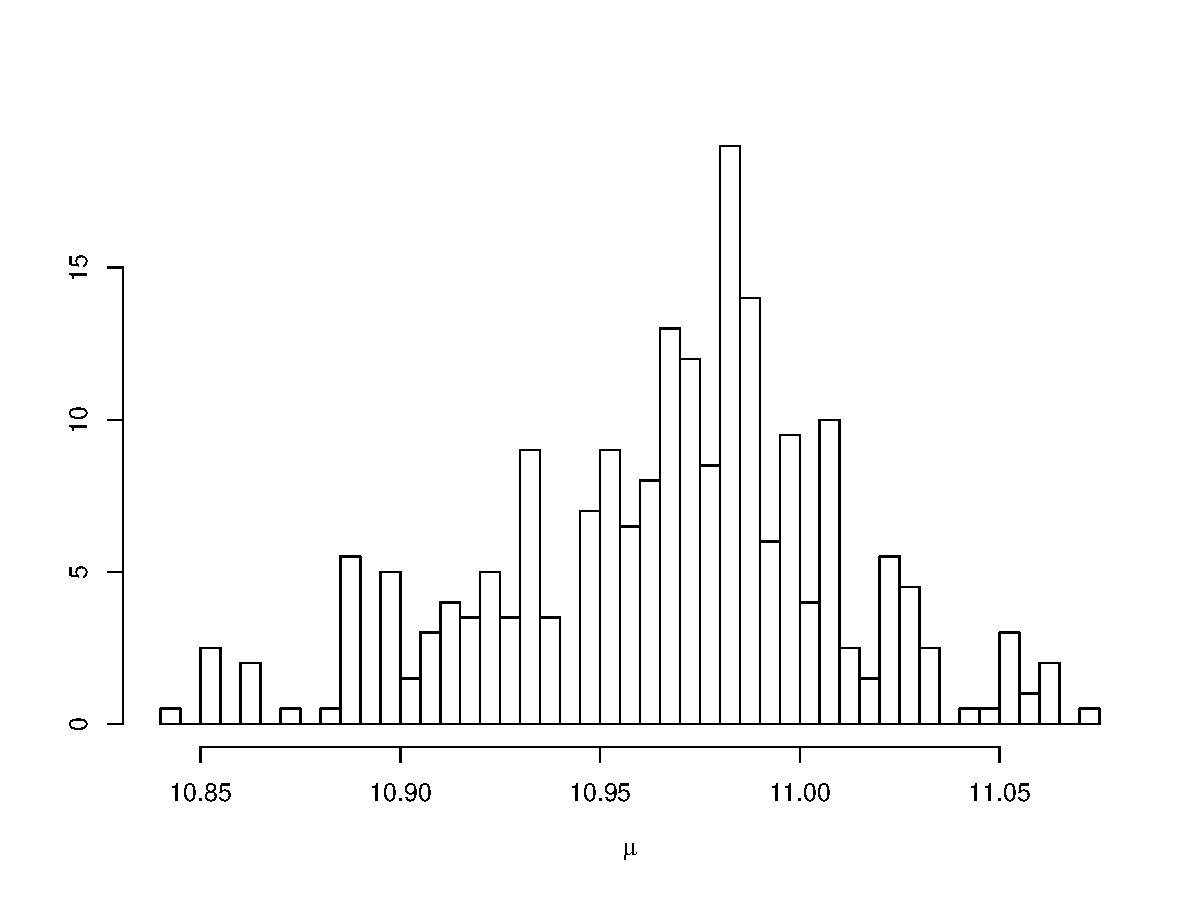
\includegraphics[scale=0.4]{figuras/mu_mh_500.pdf}}}%
	\qquad
	\subfloat[Histograma de $\sigma^2$]{{
			\label{fig:s2_mh_500}
			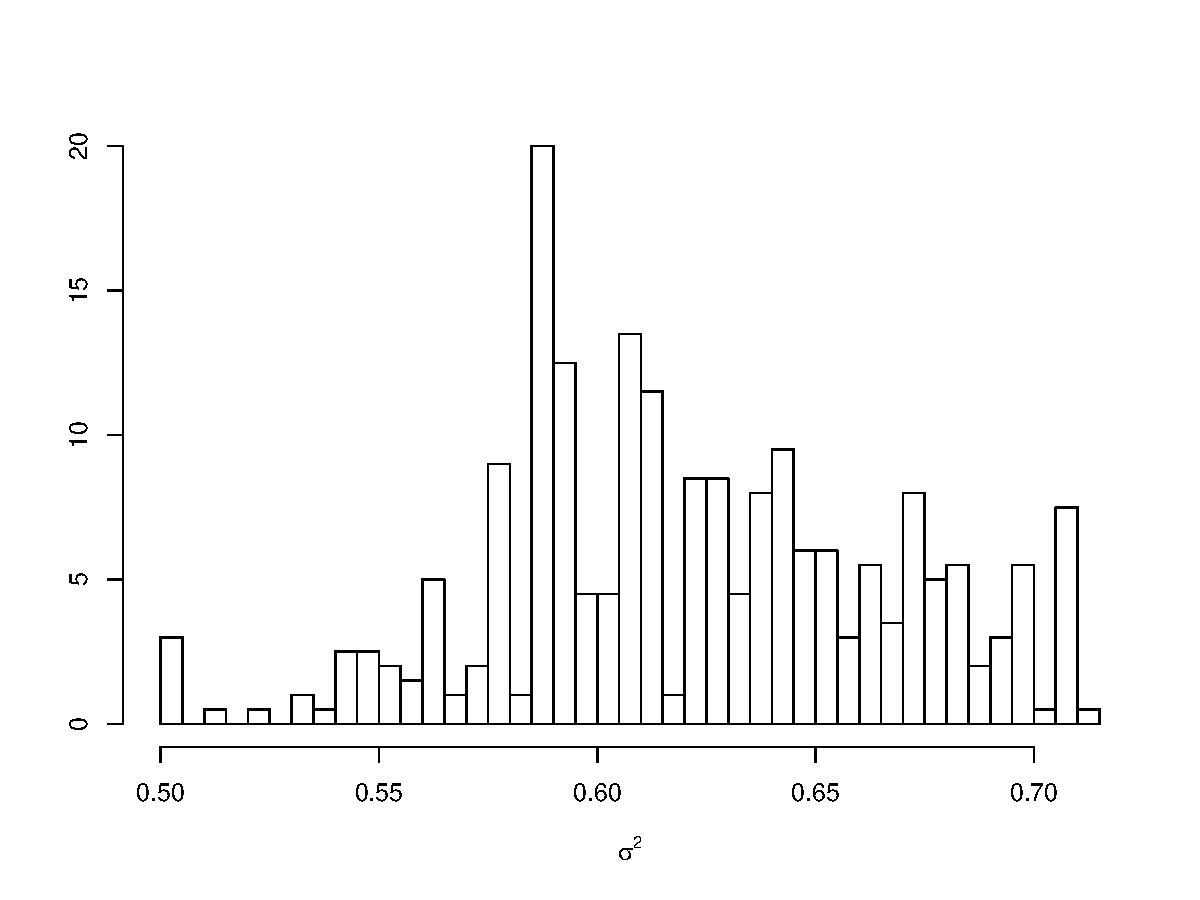
\includegraphics[scale=0.4]{figuras/s2_mh_500.pdf}}}%
	\subfloat[Histograma de $\nu$]{{
			\label{fig:nu_mh_500}
			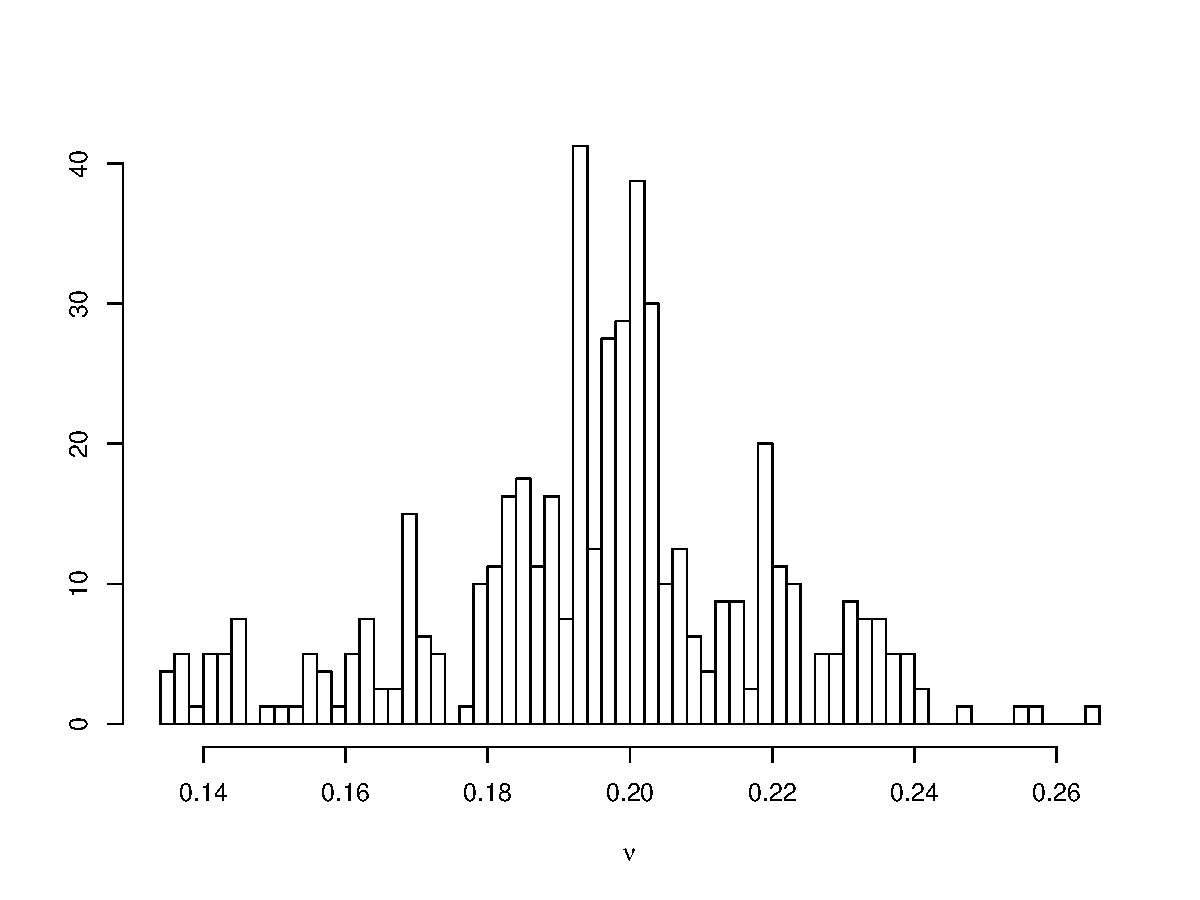
\includegraphics[scale=0.4]{figuras/nu_mh_500.pdf}}}%
	\caption{Histograma das densidades \textit{a posteriori} marginais pelo método MCMC--MH, $k = 500$}%
\end{figure}

\begin{figure}[t]%
	\centering
	\subfloat[Histograma de $\mu$]{{
			\label{fig:mu_mh_5000}
			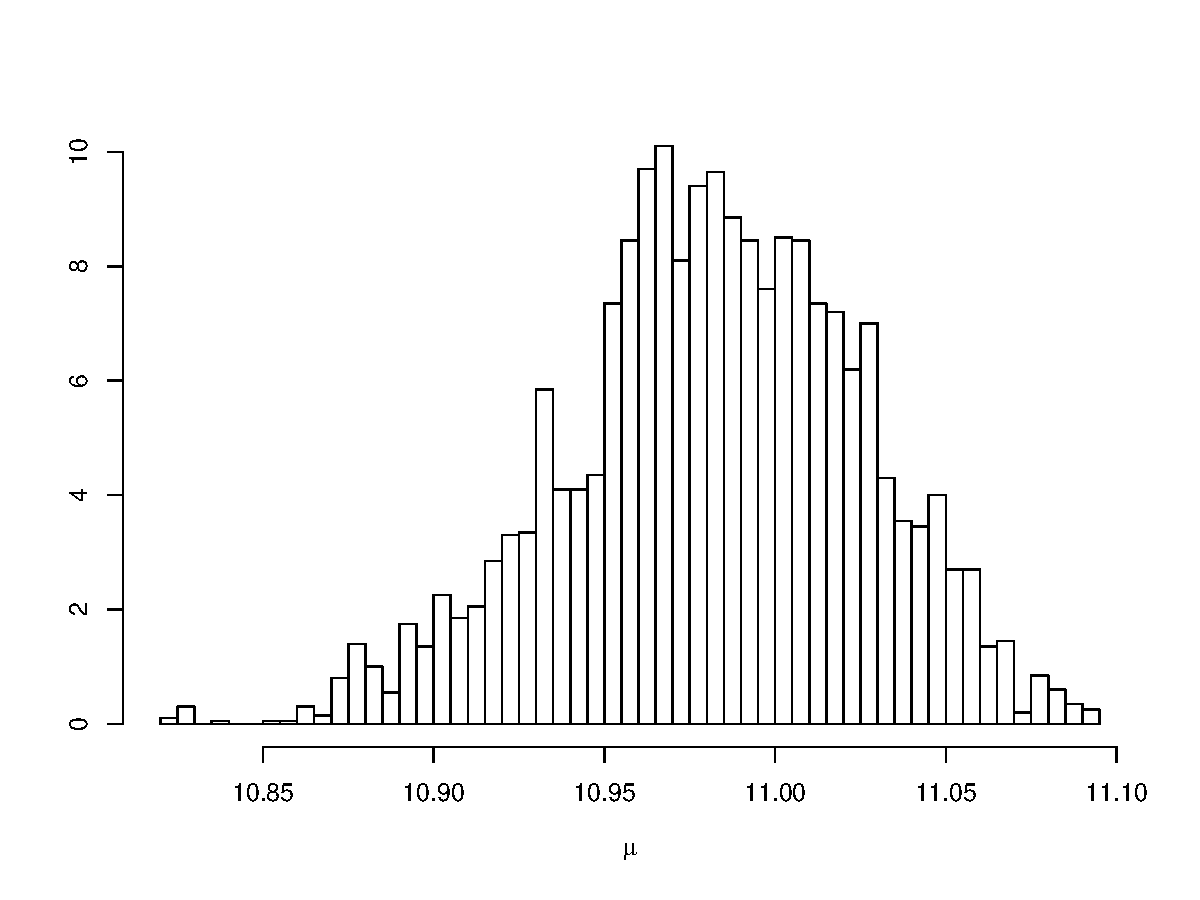
\includegraphics[scale=0.4]{figuras/mu_mh_5000.pdf}}}%
	\qquad
	\subfloat[Histograma de $\sigma^2$]{{
			\label{fig:s2_mh_5000}
			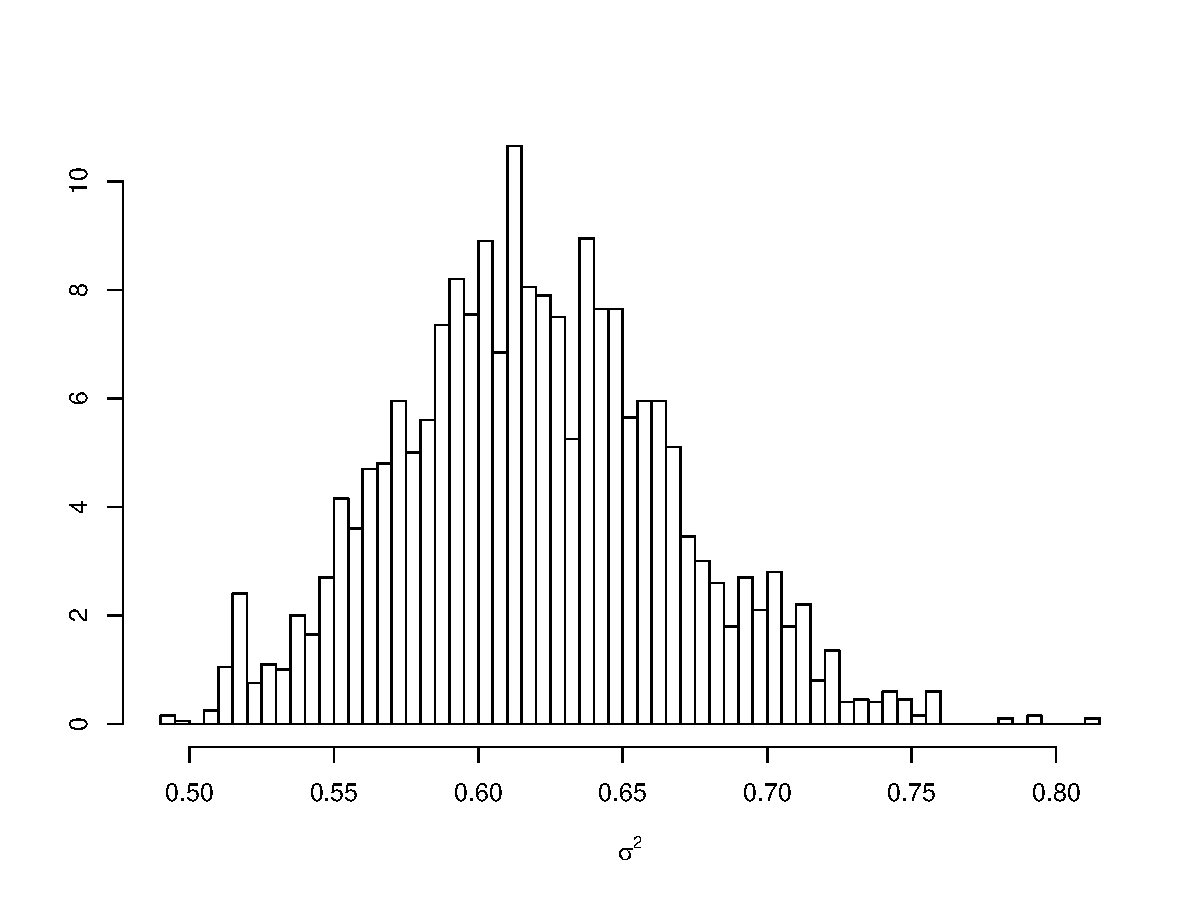
\includegraphics[scale=0.4]{figuras/s2_mh_5000.pdf}}}%
	\subfloat[Histograma de $\nu$]{{
			\label{fig:nu_mh_5000}
			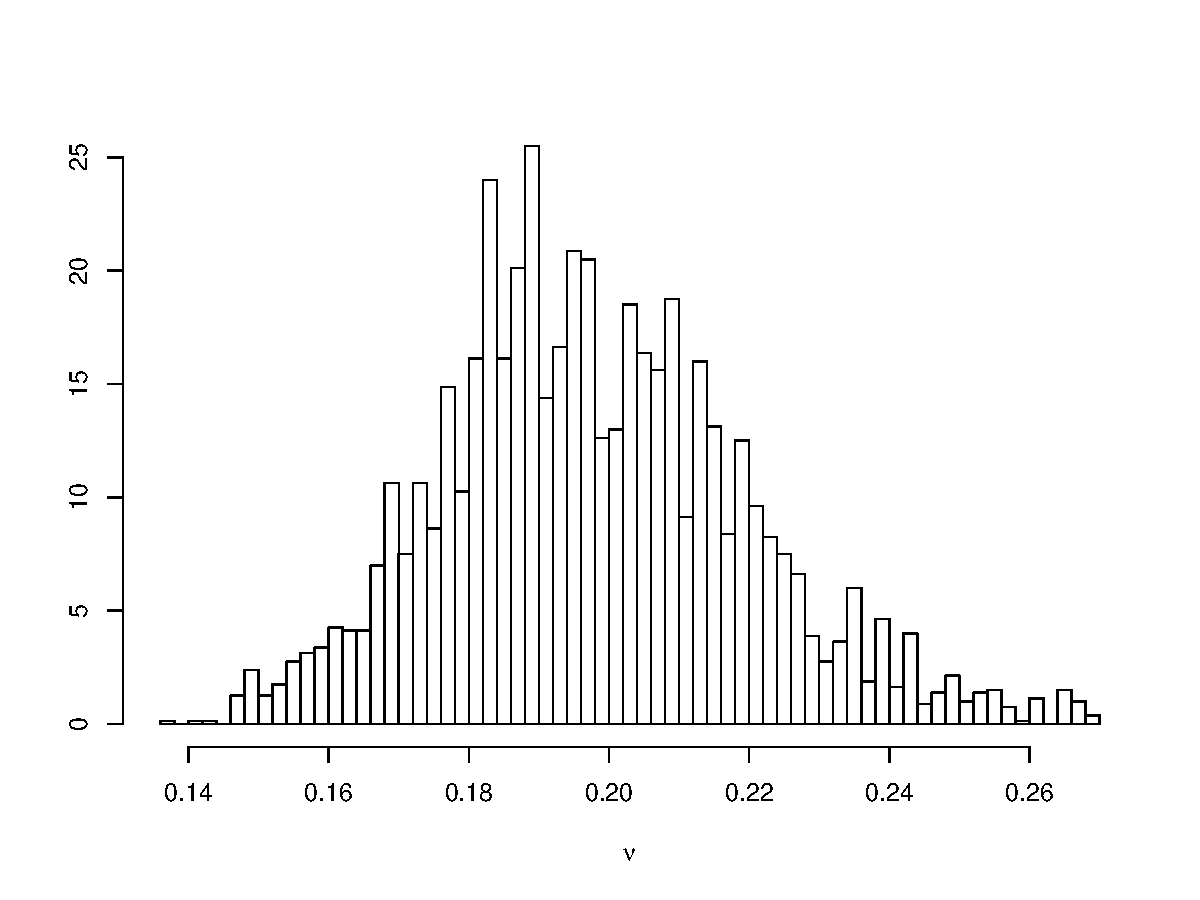
\includegraphics[scale=0.4]{figuras/nu_mh_5000.pdf}}}%
	\caption{Histograma das densidades \textit{a posteriori} marginais pela método MCMC--MH, $k = 5000$}%
\end{figure}

\begin{figure}[t]%
	\centering
	\subfloat[Histograma de $\mu$]{{
			\label{fig:mu_mh_50000}
			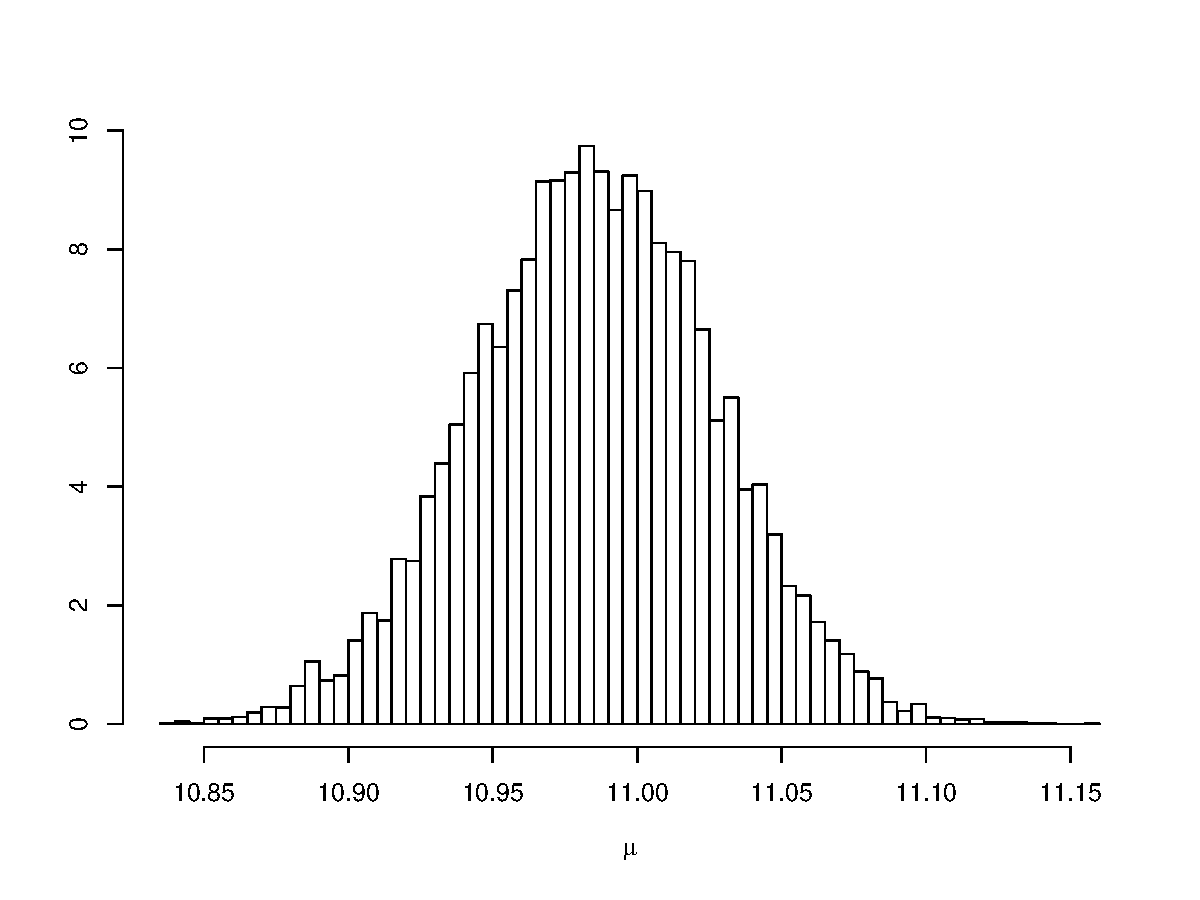
\includegraphics[scale=0.4]{figuras/mu_mh_50000.pdf}}}%
	\qquad
	\subfloat[Histograma de $\sigma^2$]{{
			\label{fig:s2_mh_50000}
			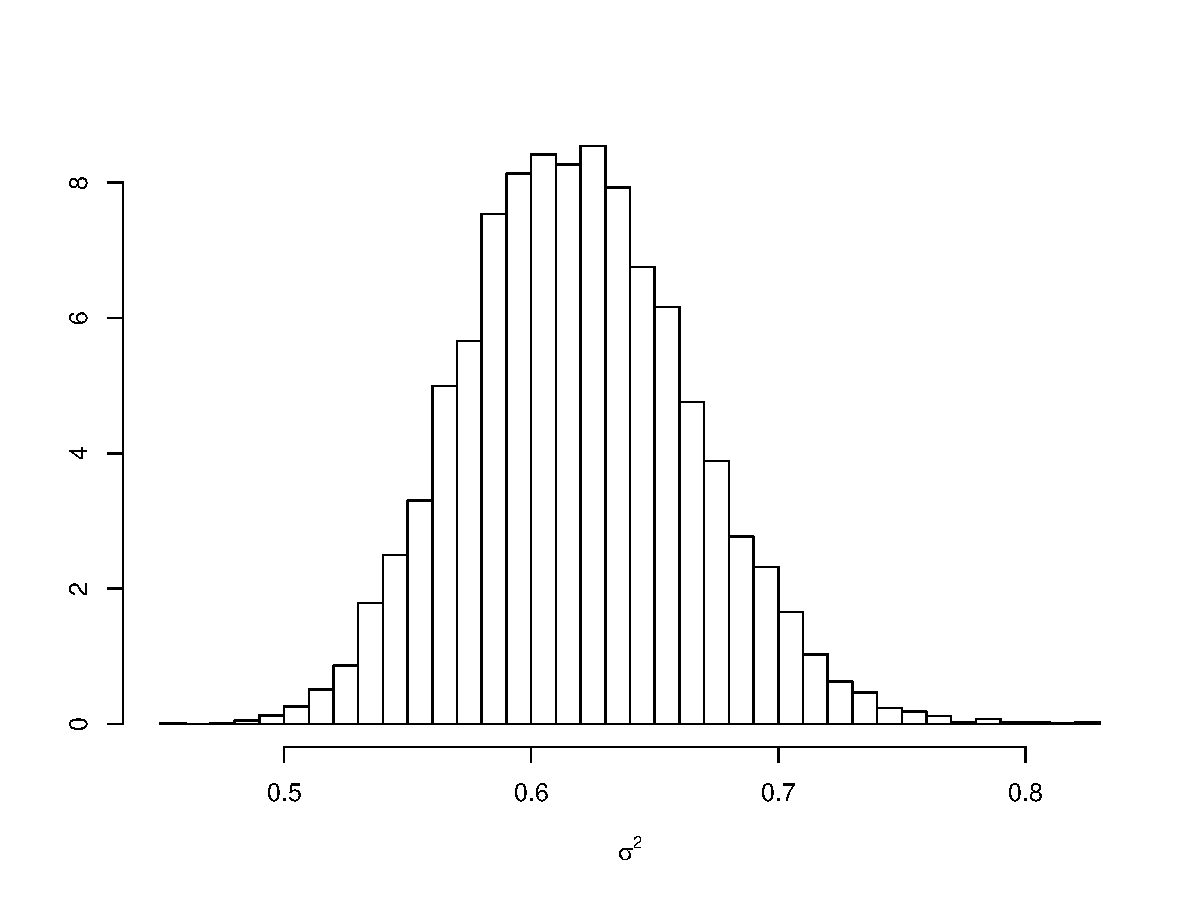
\includegraphics[scale=0.4]{figuras/s2_mh_50000.pdf}}}%
	\subfloat[Histograma de $\nu$]{{
			\label{fig:nu_mh_50000}
			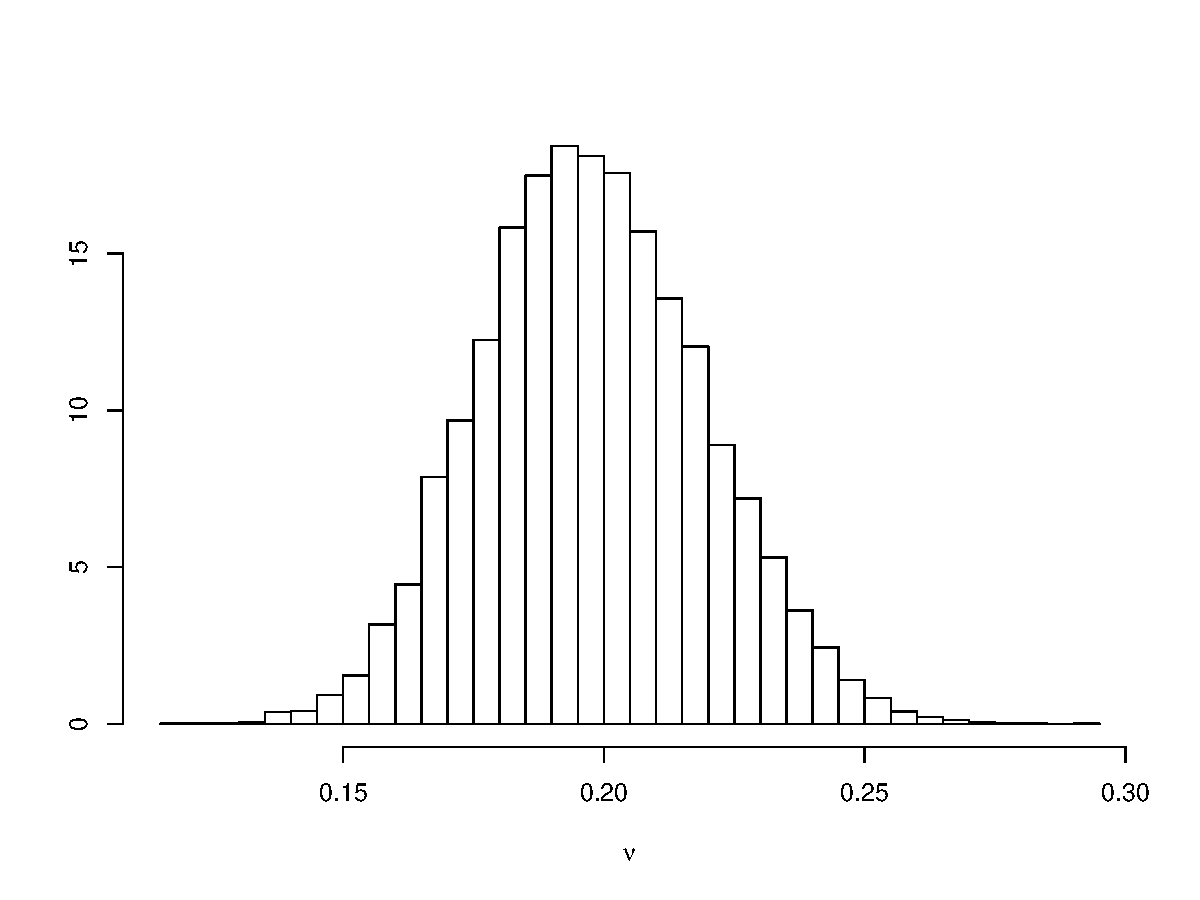
\includegraphics[scale=0.4]{figuras/nu_mh_50000.pdf}}}%
	\caption{Histograma das densidades \textit{a posteriori} marginais pela método MCMC--MH, $k = 50000$}%
\end{figure}

No presente trabalho, deseja-se amostrar os parâmetros $\mu, \sigma^2$ e $\nu$ da distribuição \textit{a posteriori} $p(\mu, \sigma^2, \nu | \bm{x})$ do modelo de mistura finita de normais com variância contaminada. O uso do algoritmo MH para cada uma das 3 cadeias correspondentes se justifica pelo fato de que: (i) em nenhum dos parâmetros é possível obter analiticamente a respectiva distribuição condicional completa, de modo que será necessário amostrar da distribuição \textit{a posteriori} conjunta, e (ii) como a distribuição \textit{a posteriori} conjunta é escrita como o produto de uma constante de proporcionalidade vezes um núcleo que depende dos parâmetros, o algoritmo MH continua válido quando se trabalha com o núcleo do lado direito de \eqref{eq:dist_post} no lugar de $p(\mu, \sigma^2, \nu | \bm{x})$. Novamente, para avaliar este núcleo, toma-se a soma do logaritmo de todas as quantidades que o compõem quando multiplicadas entre si. Assim como feito no método SIR, para a distribuição proposta $q(\cdot)$ também será escolhida uma normal trivariada $N_3(\bm{\mu}, \bm{\Sigma})$ e a mesma reparametrização para $(\mu, \sigma^2, \nu)$ será reutilizada de modo a garantir que a distribuição proposta gere adequadamente de $p(\mu, \sigma^2, \nu | \bm{x})$ pelo algoritmo MH, inclusive com os mesmos valores do vetor de médias $\bm{\mu} = (\mu, \log(\sigma^2), \log[\nu/(1-\nu)]) = (11, \log(0.64), \log[0.2/0.8])$ e da matriz de covariância $\bm{\Sigma} = \textrm{diag}\{0.0022, 0.0065, 0.0203\}$.

Para aplicar o método MCMC com algoritmo MH de modo a obter amostras \textit{a posteriori} de $\mu$, $\sigma^2$ e $\nu$, foram considerados 3 cenários: $k = \{500, 5000, 50000\}$, os mesmos do método SIR. Como no MCMC é necessário definir um estado inicial da cadeia, em geral com densidade conjunta muito baixa, escolheu-se o ponto $y^{(1)}gaussia = (10.86, log(0.50), log(0.14/0.86))$ para inicialização do algoritmo, com logaritmo do núcleo da \textit{posteriori} avaliado em $1.760 \times 10^{-235}$, ainda numericamente não nulo pelo \textit{R}. Evidentemente, as primeiras amostras geradas não terão distribuição próxima à da limite, razão pela qual será feito um descarte (em inglês, \textit{burn-in}) de 20\% a partir dos valores iniciais. Logo, ao final se terão $400, 4000$ e $40000$ valores gerados nos cenários correspondentes. Como o vetor de valores uniformes para comparação das probabilidades de aceitação a cada passo não dependem dos valores gerados de $q$, em todos os cenários eles foram construídos fora da rotina iterativa do algoritmo MH. No final, as taxas de aceitação das amostras propostas ficaram em $45.2\%$; $40.42\%$ e $41.11\%$ para os cenários em ordem crescente de tamanho da cadeia. Nas figuras \ref{fig:mu_mh_500} a \ref{fig:nu_mh_500}; \ref{fig:mu_mh_5000} a \ref{fig:nu_mh_5000} e \ref{fig:mu_mh_50000} a \ref{fig:nu_mh_50000} são apresentados os histogramas para as amostras \textit{a posteriori} de cada parâmetro por cenário.

Para $k=500$, a aproximação da densidade não é boa para nenhum dos 3 parâmetros com as $400$ amostras restantes: há pontos extremos distantes do que seria a massa principal, especialmente para $\nu$. Além disso, há várias modas locais, indicando uma curva que está longe de ser suave. Entretanto, é possível dizer já neste cenário como é o comportamento de cada parâmetro com relação à locação, assim como no método SIR.

Para $k=5000$, a aproximação é bem mais suave e há menos \textit{outliers} quando consideradas as $4000$ amostras restantes. O número de modas locais também é reduzido em comparação ao cenário anterior, embora esta quantidade ainda seja moderada para $\sigma^2$ e alta para $\nu$. Além do comportamento com relação à locação, é possível dizer também como é o comportamento com relação à dispersão da densidade \textit{a posteriori} marginal de cada parâmetro, mas não com relação à assimetria, ao contrário do método SIR.

Para $k=50000$, os gráficos confirmam a tendência apresentada pelo cenário anterior, mas com uma suavização ainda melhor, embora não tão boa quanto no algoritmo SIR para a mesma quantidade de amostras \textit{a posteriori} geradas, mesmo com o \textit{burn-in} de 20\% das amostras. Isso se pelo fato de que o começo da cadeia é fortemente influenciada pela escolha do valor inicial mesmo com o \textit{burn-in}, mas essa influência vai diminuindo ao longo dos passos do algoritmo. Todas as distribuições são praticamente unimodais (há algumas modas locais quase imperceptíveis nos gráficos de $\mu$ e $\sigma^2$) e praticamente não há mais \textit{outliers}. Agora, é possível identificar uma leve assimetria à direita nos gráficos de $\sigma^2$ e $\nu$.

Obtidas as amostras \textit{a posteriori} marginais de cada parâmetro, para aproximar as estatísticas de média, variância, assimetria e curtose novamente serão tomadas as respectivas estimativas amostrais. Na Tabela \ref{tab3}, são apresentados os valores aproximados para tais estatísticas em cada um dos três cenários.

\begin{table}[htb]
	\caption{Estatísticas \textit{a posteriori} para $(\mu, \sigma^2, \nu)$ pelo método MCMC--MH}
	\label{tab3}
	\centering
	\begin{tabular}{cccccc}
		\toprule
		Cenário & Parâmetro & Média & Variância & Assimetria & Curtose \\
		\midrule
		$k = 500$ & $\mu$ & 10.9672 & 0.0018 & -0.3768 & 3.2193 \\
		& $\sigma^2$ & 0.6226 & 0.0020 & -0.0684 & 2.6117 \\
		& $\nu$      & 0.1957 & 0.0006 & -0.3313 & 3.2991 \\
		\midrule
		$k = 5000$ & $\mu$ & 10.9818 & 0.0019 & -0.2466 & 2.9894 \\
		& $\sigma^2$ & 0.6197 & 0.0023 & 0.2372 & 3.0057 \\
		& $\nu$      & 0.1977 & 0.0005 & 0.3878 & 3.2038 \\
		\midrule
		$k = 50000$ & $\mu$ & 10.9852 & 0.0017 & -0.0272 & 2.9451 \\
		& $\sigma^2$ & 0.6188 & 0.0021 & 0.2472 & 3.1088 \\
		& $\nu$      & 0.1978 & 0.0005 & 0.1331 & 2.8971 \\
		\bottomrule
	\end{tabular}
\end{table}

Pela Tabela \ref{tab3}, pode-se concluir que tanto a média quanto a variância \textit{a posteriori} variaram muito pouco nos três cenários, independente do parâmetro considerado. Logo, amostras \textit{a posteriori} de tamanho moderado são o suficiente para se obter uma boa aproximação destas duas estatísticas. Por outro lado, o mesmo não pode ser dito para a assimetria e curtose \textit{a posteriori}, para as quais há grandes mudanças inclusive na primeira casa decimal, mesmo de $k=5000$ para $k=50000$, assim como no método SIR (Tabela \ref{tab2}). Apesar deste fato, no método MCMC com passos MH também se pode dizer que houve uma estabilidade nas aproximações destas duas últimas estatísticas na medida em que $k$ crescia, embora com convergência mais lenta do que no método SIR.

Com relação aos valores em si, as médias \textit{a posteriori} para os 3 parâmetros ficaram muito próximas dos respectivos valores do modelo para a distribuição amostral, embora não tanto quanto no método SIR. Para as variâncias \textit{a posteriori}, todas elas foram bem pequenas, em especial para $\nu$, assim como na quadratura e no SIR. Com relação à assimetria \textit{a posteriori}, esta foi praticamente nula para $\mu$ e positiva, mas fraca, para $\sigma^2$ e $\nu$ (um pouco mais forte para a primeira, assim como na quadratura e diferente do método SIR). Por fim, as aproximações para a curtose \textit{a posteriori} foram todas bem próximas de 3 (em geral, acima deste valor), com o parâmetro $\mu$ mais próximo desse valor e $\sigma^2$ o mais afastado, a mesma conclusão na quadratura.

Por fim, no Anexo são apresentados os gráficos de convergência (traço) e de autocorrelação das 9 cadeias geradas (3 para cada cenário, correspondentes a cada parâmetro), nas figuras \ref{fig:trace_mu_mh} a \ref{fig:acf_nu_mh}. Para todos os parâmetros, podemos dizer que houve convergência para a distribuição limite, o que fica bastante evidentemente no cenário $k = 50000$. Com relação à autocorrelação, é necessário uma defasagem (em inglês, \textit{lag}) moderada, de tamanho pelo menos igual a 20, para remover a autocorrelação dentro da cadeia. Como $k$ é grande se comparado a este valor em todos os cenários, isto afetará pouco nas estimativas de variância \textit{a posteriori} para cada parâmetro.

\section{Considerações Finais}\label{consfin}

%Texto descrevendo de forma resumida o que foi feito nas seções anteriores, bem como os resultados dos métodos quanto à convergência, à medida que se aumenta o tamanho amostral m da distribuição \textit{a poseteriori}.

\bibliographystyle{unsrt}
\bibliography{ref}

\newpage

\section*{Apêndice: Código R para os Resultados Apresentados}

\subsection*{Introdução}

\begin{verbatim}
# Tamanho amostral "n"; parâmetros "mu", "s2" (sigma^2) e "nu" do modelo para
# a distribuição amostral e hiperparâmetros m, V, a e d das distribuições "a
# priori" (somente para "mu" e "s2"):

n = 500; mu = 11; s2 = 0.64; nu = 0.2; m = 11; V = 1; a = 7; d = 4

# Geração hierárquica da amostra de tamanho "n" do modelo:

U_pdf = function(n, nu) {
	u = sample(c(100, 1), prob=c(nu, 1-nu), size=n, replace=T)
}

set.seed(122019)

u = U_pdf(n, nu)
sam = rnorm(n, mu, sqrt(s2*u))

# Histograma e estatísticas da amostra gerada do modelo (figura 1):

par(mar = c(5,5,3,2))
hist(sam, breaks=100, prob=T, main="", xlim = c(-10, 40), ylim = c(0, 0.5),
	 xlab = "Amostra do modelo", ylab = "Densidade empírica")
library(moments); mean(sam); var(sam); skewness(sam); kurtosis(sam)

# Cálculo do logaritmo do núcleo da distribuição "a posteriori" original:

logA = function(X, mu, sigma2, nu) {
	n = length(X)
	k1 = (nu/10)*exp(-(X-mu)^2/(2*100*sigma2))
	k2 = (1-nu)*exp(-(X-mu)^2/(2*sigma2))
	k = log(k1 + k2)
	return(k)
}

logh = function(n, mu, sigma2, nu, m, V, a, d) {
	k1 = -((n + 1)/2 + a + 1)*log(sigma2)
	k2 = -((mu - m)^2/(2*V) + d)/sigma2
	k = k1 + k2
	return(k)
}

logkpost = function(X, mu, sigma2, nu, m, V, a, d) {
	n = length(X)
	lA = logA(X, mu, sigma2, nu)
	lh = logh(n, mu, sigma2, nu, m, V, a, d)
	lkp = sum(lA) + lh
	return(lkp)}

# Gráficos dos intervalos de massa probabilística para cada parâmetro do
# núcleo da distribuição "a posteriori", fixados os demais, após algumas
# tentativas anteriores para redução dos limites do gráfico e melhor vi-
# sualização da curva (figuras 2a a 2c):

mu_sup=seq(10.8, 11.2, 0.001); t_mu=length(mu_sup); kp_mu=numeric(t_mu)

for(i in 1:t_mu) {
	kp_mu[i] = exp(logkpost(X=sam,
	mu=mu_sup[i], sigma2=s2, nu=nu, m=m, V=V, a=a, d=d))
	}
plot(mu_sup, kp_mu, type="l", main="",
     xlab=expression(paste(mu)), ylab="")

s2_sup=seq(0.4, 0.8, 0.001); t_s2=length(s2_sup); kp_s2=numeric(t_s2)

for(i in 1:t_s2) {
	kp_s2[i] = exp(logkpost(X=sam,
	mu=mu, sigma2=s2_sup[i], nu=nu, m=m, V=V, a=a, d=d))
	}
plot(s2_sup, kp_s2, type="l", main="",
	 xlab=expression(paste(sigma^2)), ylab="")

nu_sup=seq(0.1, 0.3, 0.001); t_nu=length(nu_sup); kp_nu=numeric(t_nu)

for(i in 1:t_nu) {
	kp_nu[i] = exp(logkpost(X=sam,
	mu=mu, sigma2=s2, nu=nu_sup[i], m=m, V=V, a=a, d=d))
	}
plot(nu_sup, kp_nu, type="l", main="",
     xlab=expression(paste(nu)), ylab="")
\end{verbatim}

\subsection*{O Método da Quadratura de Riemann}

\begin{verbatim}

# Cenários considerados, variando no número de subintervalos utilizados:

L1 = 15; L2 = 50; L3 = 100

# Tamanhos dos subintervalos, dada a combinação de cenário e parâmetro, e
# grades definidas pelos mesmos:

mu_step1 = (11.13 - 10.85)/L1; mu_gr1 = seq(10.85, 11.13, mu_step1)
mu_step2 = (11.13 - 10.85)/L2; mu_gr2 = seq(10.85, 11.13, mu_step2)
mu_step3 = (11.13 - 10.85)/L3; mu_gr3 = seq(10.85, 11.13, mu_step3)

s2_step1 = (0.78 - 0.48)/L1; s2_gr1 = seq(0.48, 0.78, s2_step1)
s2_step2 = (0.78 - 0.48)/L2; s2_gr2 = seq(0.48, 0.78, s2_step2)
s2_step3 = (0.78 - 0.48)/L3; s2_gr3 = seq(0.48, 0.78, s2_step3)

nu_step1 = (0.26 - 0.13)/L1; nu_gr1 = seq(0.13, 0.26, nu_step1)
nu_step2 = (0.26 - 0.13)/L2; nu_gr2 = seq(0.13, 0.26, nu_step2)
nu_step3 = (0.26 - 0.13)/L3; nu_gr3 = seq(0.13, 0.26, nu_step3)

# Combinando as três grades unidimensionais em cada cenário, todas com
# número igual de subintervalos e de pontos (nos limites dos interval-
# os) para integração numérica:

grid_tri1 = cbind(mu_gr1, s2_gr1, nu_gr1); l1 = nrow(grid_tri1)
grid_tri2 = cbind(mu_gr2, s2_gr2, nu_gr2); l2 = nrow(grid_tri2)
grid_tri3 = cbind(mu_gr3, s2_gr3, nu_gr3); l3 = nrow(grid_tri3)

# Produto triplo dos tamanhos dos subintervalos em cada cenário:

prod_step1 = mu_step1*s2_step1*nu_step1
prod_step2 = mu_step2*s2_step2*nu_step2
prod_step3 = mu_step3*s2_step3*nu_step3

# Cálculo do inverso da constante de proporcionalidade em cada cenário:

cprop = function(l, X, mgr, s2gr, ngr, prst, m, V, a, d) {
	c = 0
	for (i in 1:l) {
		for (j in 1:l) {
			for (k in 1:l) {
				aux = logkpost(X, mgr[i], s2gr[j], ngr[k], m, V, a, d)
				c = c + exp(aux)*prst
			}
		}
	}
	return(c)
}

c1 = cprop(l=l1, X=sam, mgr=mu_gr1, s2gr=s2_gr1, ngr=nu_gr1,
		   prst=prod_step1, m=m, V=V, a=a, d=d)
c2 = cprop(l=l2, X=sam, mgr=mu_gr2, s2gr=s2_gr2, ngr=nu_gr2,
		   prst=prod_step2, m=m, V=V, a=a, d=d)
c3 = cprop(l=l3, X=sam, mgr=mu_gr3, s2gr=s2_gr3, ngr=nu_gr3,
		   prst=prod_step3, m=m, V=V, a=a, d=d)
c1; c2; c3

# Cálculo das densidades "a posteriori" marginais em cada cenário, com
# uso do produto duplo dos tamanhos dos subintervalos em cada cenário:

pr1_dup12 = mu_step1*s2_step1
pr1_dup13 = mu_step1*nu_step1
pr1_dup23 = s2_step1*nu_step1
\end{verbatim}

\newpage

\begin{verbatim}
pr2_dup12 = mu_step2*s2_step2
pr2_dup13 = mu_step2*nu_step2
pr2_dup23 = s2_step2*nu_step2

pr3_dup12 = mu_step3*s2_step3
pr3_dup13 = mu_step3*nu_step3
pr3_dup23 = s2_step3*nu_step3

postmu_quarie = function(l, X, mgr, s2gr, ngr, prst, m, V, a, d, c) {
	postmu = numeric(l)
	for (i in 1:l) {
		postconj = 0
		for (j in 1:l) {
			for(k in 1:l) {
				aux = logkpost(X, mgr[i], s2gr[j], ngr[k], m, V, a, d)
				postconj = postconj + exp(aux)*prst
			}
		}
		postmu[i] = postconj/c
	}
	return(postmu)
}

pmq1 = postmu_quarie(l=l1, X=sam, mgr=mu_gr1, s2gr=s2_gr1, ngr=nu_gr1,
					 prst=pr1_dup23, m=m, V=V, a=a, d=d, c=c1)
pmq2 = postmu_quarie(l=l2, X=sam, mgr=mu_gr2, s2gr=s2_gr2, ngr=nu_gr2,
					 prst=pr2_dup23, m=m, V=V, a=a, d=d, c=c2)
pmq3 = postmu_quarie(l=l3, X=sam, mgr=mu_gr3, s2gr=s2_gr3, ngr=nu_gr3,
					 prst=pr3_dup23, m=m, V=V, a=a, d=d, c=c3)

plot(mu_gr1,pmq1,type="l",main="",xlab=expression(paste(mu)),ylab="")
plot(mu_gr2,pmq2,type="l",main="",xlab=expression(paste(mu)),ylab="")
plot(mu_gr3,pmq3,type="l",main="",xlab=expression(paste(mu)),ylab="")

posts2_quarie = function(l, X, mgr, s2gr, ngr, prst, m, V, a, d, c) {
	posts2 = numeric(l)
	for (i in 1:l) {
		postconj = 0
		for (j in 1:l) {
			for(k in 1:l) {
				aux = logkpost(X, mgr[j], s2gr[i], ngr[k], m, V, a, d)
				postconj = postconj + exp(aux)*prst
			}
		}
		posts2[i] = postconj/c
	}
	return(posts2)
}

\end{verbatim}

\newpage

\begin{verbatim}
psq1 = posts2_quarie(l=l1, X=sam, mgr=mu_gr1, s2gr=s2_gr1, ngr=nu_gr1,
					 prst=pr1_dup13, m=m, V=V, a=a, d=d, c=c1)
psq2 = posts2_quarie(l=l2, X=sam, mgr=mu_gr2, s2gr=s2_gr2, ngr=nu_gr2,
					 prst=pr2_dup13, m=m, V=V, a=a, d=d, c=c2)
psq3 = posts2_quarie(l=l3, X=sam, mgr=mu_gr3, s2gr=s2_gr3, ngr=nu_gr3,
					 prst=pr3_dup13, m=m, V=V, a=a, d=d, c=c3)

plot(s2_gr1, psq1, type="l", main="", xlab=expression(paste(sigma^2)),
	 ylab="")
plot(s2_gr2, psq2, type="l", main="", xlab=expression(paste(sigma^2)),
	 ylab="")
plot(s2_gr3, psq3, type="l", main="", xlab=expression(paste(sigma^2)), 
	 ylab="")

postnu_quarie = function(l, X, mgr, s2gr, ngr, prst, m, V, a, d, c) {
	postnu = numeric(l)
	for (i in 1:l) {
		postconj = 0
		for (j in 1:l) {
			for(k in 1:l) {
				aux = logkpost(X, mgr[j], s2gr[k], ngr[i], m, V, a, d)
				postconj = postconj + exp(aux)*prst
			}
		}
		postnu[i] = postconj/c
	}
	return(postnu)
}

pnq1 = postnu_quarie(l=l1, X=sam, mgr=mu_gr1, s2gr=s2_gr1, ngr=nu_gr1,
					 prst=pr1_dup12, m=m, V=V, a=a, d=d, c=c1)
pnq2 = postnu_quarie(l=l2, X=sam, mgr=mu_gr2, s2gr=s2_gr2, ngr=nu_gr2,
					 prst=pr2_dup12, m=m, V=V, a=a, d=d, c=c2)
pnq3 = postnu_quarie(l=l3, X=sam, mgr=mu_gr3, s2gr=s2_gr3, ngr=nu_gr3,
					 prst=pr3_dup12, m=m, V=V, a=a, d=d, c=c3)

plot(nu_gr1,pnq1,type="l",main="",xlab=expression(paste(nu)),ylab="")
plot(nu_gr2,pnq2,type="l",main="",xlab=expression(paste(nu)),ylab="")
plot(nu_gr3,pnq3,type="l",main="",xlab=expression(paste(nu)),ylab="")
\end{verbatim}

\newpage

\begin{verbatim}
# Cálculo da média, variância, assimetria e curtose "a posteriori" para
# cada parâmetro:

stat_post = function(gr, marg, prst) {
	media = 0
	var = 0
	assim = 0
	cur = 0
	l = length(gr)
	
	aux1 = sum(gr*marg*prst)     # Aproxima 1º momento.
	aux2 = sum((gr^2)*marg*prst) # Aproxima 2º momento.
	aux3 = sum((gr^3)*marg*prst) # Aproxima 3º momento.
	aux4 = sum((gr^4)*marg*prst) # Aproxima 4º momento.
	
	media = aux1
	var = aux2 - (media)^2
	assim = (aux3 - 3*media*var - media^3)/(var^(3/2))
	cur = (aux4 - 4*media*aux3 + 6*media^2*aux2 - 3*(media^4))/(var^2)
	return(list(media, var, assim, cur))
}

stat_post(mu_gr1, pmq1, mu_step1)
stat_post(mu_gr2, pmq2, mu_step2)
stat_post(mu_gr3, pmq3, mu_step3)

stat_post(s2_gr1, psq1, s2_step1)
stat_post(s2_gr2, psq2, s2_step2)
stat_post(s2_gr3, psq3, s2_step3)

stat_post(nu_gr1, pnq1, nu_step1)
stat_post(nu_gr2, pnq2, nu_step2)
stat_post(nu_gr3, pnq3, nu_step3)

\end{verbatim}

\subsection*{O Método da Reamostragem Por Importância Sequencial (SIR)}

\begin{verbatim}
# Cálculo do logaritmo do núcleo da distribuição "a posteriori" reparametrizada:

logr = function(sigma2, nu) {
k = log(sigma2) + 3*log(nu) - log(1-nu)
return(k)
}
\end{verbatim}

\newpage

\begin{verbatim}
logkpost_re = function(X, mu, sigma2, nu, m, V, a, d) {
n = length(X)
lA = logA(X, mu, sigma2, nu)
lh = logh(n, mu, sigma2, nu, m, V, a, d)
lr = logr(sigma2, nu)
lkrp = sum(lA) + lh + lr
return(lkrp)
}

logkpost_re(sam, mu, s2, nu, m, V, a, d)

# Cenários de tamanhos do vetor de pesos e de amostras "a posteriori" via SIR:

aw1 = 5000; aw2 = 50000; aw3 = 500000
am1 = aw1/10; am2 = aw2/10; am3 = aw3/10

# Valores reparametrizados da diagonal principal da matriz de covariâncias
# da distribuição normal trivariada:

((11.13-10.85)/6)^2
((log(0.78)-log(0.48))/6)^2
((log(0.26/0.74)-log(0.13/0.87))/6)^2

# Geração de amostras da distribuição normal trivariada:

library(mvtnorm)

set.seed(122019)
r1_q = rmvnorm(aw1, mean=c(11, log(0.64), log(0.2/0.8)),
			   sigma=diag(c(0.0022, 0.0065, 0.0203)))
set.seed(122019)
r2_q = rmvnorm(aw2, mean=c(11, log(0.64), log(0.2/0.8)),
			   sigma=diag(c(0.0022, 0.0065, 0.0203)))
set.seed(122019)
r3_q = rmvnorm(aw3, mean=c(11, log(0.64), log(0.2/0.8)),
			   sigma=diag(c(0.0022, 0.0065, 0.0203)))

# Cálculo da densidade para cada ponto das amostras geradas:

d1_q = dmvnorm(r1_q, mean=c(11, log(0.64), log(0.2/0.8)), sigma=diag(3))
d2_q = dmvnorm(r2_q, mean=c(11, log(0.64), log(0.2/0.8)), sigma=diag(3))
d3_q = dmvnorm(r3_q, mean=c(11, log(0.64), log(0.2/0.8)), sigma=diag(3))
\end{verbatim}

\newpage

\begin{verbatim}
# Cálculo dos pesos de reamostragem:

weiSIR = function(X, r_q, m, V, a, d, d_q) {
	k = nrow(r_q)
	aux1 = aux2 = w = numeric(k)
	for(i in 1:k) {
		aux1[i] = logkpost_re(X=X, mu=r_q[i,1], sigma2=exp(r_q[i,2]),
							  nu=1/(1+exp(-r_q[i,3])), m=m, V=V, a=a,
							  d=d)
	}
	aux2 = aux1/d_q
	w = aux2/sum(aux2)
	return(w)
}

w1 = weiSIR(sam, r1_q, m, V, a, d, d1_q); sum(w1)
w2 = weiSIR(sam, r2_q, m, V, a, d, d2_q); sum(w2)
w3 = weiSIR(sam, r3_q, m, V, a, d, d3_q); sum(w3)

# Geração das amostras da densidade aproximada pelo método SIR com os pesos
# calculados acima:

set.seed(122019)
am1_mu_p = sample(x=r1_q[,1], size=am1, replace=T, prob=w1)
set.seed(122019)
am1_s2_p = sample(x=exp(r1_q[,2]), size=am1, replace=T, prob=w1)
set.seed(122019)
am1_nu_p = sample(x=1/(1+exp(-r1_q[,3])), size=am1, replace=T, prob=w1)

set.seed(122019)
am2_mu_p = sample(x=r2_q[,1], size=am2, replace=T, prob=w2)
set.seed(122019)
am2_s2_p = sample(x=exp(r2_q[,2]), size=am2, replace=T, prob=w2)
set.seed(122019)
am2_nu_p = sample(x=1/(1+exp(-r2_q[,3])), size=am2, replace=T, prob=w2)

set.seed(122019)
am3_mu_p = sample(x=r3_q[,1], size=am3, replace=T, prob=w3)
set.seed(122019)
am3_s2_p = sample(x=exp(r3_q[,2]), size=am3, replace=T, prob=w3)
set.seed(122019)
am3_nu_p = sample(x=1/(1+exp(-r3_q[,3])), size=am3, replace=T, prob=w3)
\end{verbatim}

\newpage

\begin{verbatim}
# Média; variância; assimetria; curtose e histogramas das amostras geradas:

library(moments)

st_sam_post = function(Xpar) {
	medi = mean(Xpar)
	vari = var(Xpar)
	assi = skewness(Xpar)
	curt = kurtosis(Xpar)
	return(list(media=medi, variancia=vari, assimetria=assi, curtose=curt))
}

st_sam_post(am1_mu_p)
hist(am1_mu_p, breaks=50, prob=T, main="",
	 xlab=expression(paste(mu)), ylab="")
st_sam_post(am2_mu_p)
hist(am2_mu_p, breaks=50, prob=T, main="",
	 xlab=expression(paste(mu)), ylab="")
st_sam_post(am3_mu_p)
hist(am3_mu_p, breaks=50, prob=T, main="",
	 xlab=expression(paste(mu)), ylab="")

st_sam_post(am1_s2_p)
hist(am1_s2_p, breaks=50, prob=T, main="",
	 xlab=expression(paste(sigma^2)), ylab="")
st_sam_post(am2_s2_p)
hist(am2_s2_p, breaks=50, prob=T, main="",
	 xlab=expression(paste(sigma^2)), ylab="")
st_sam_post(am3_s2_p)
hist(am3_s2_p, breaks=50, prob=T, main="",
	 xlab=expression(paste(sigma^2)), ylab="")

st_sam_post(am1_nu_p)
hist(am1_nu_p, breaks=50, prob=T, main="",
	 xlab=expression(paste(nu)), ylab="")
st_sam_post(am2_nu_p)
hist(am2_nu_p, breaks=50, prob=T, main="",
	 xlab=expression(paste(nu)), ylab="")
st_sam_post(am3_nu_p)
hist(am3_nu_p, breaks=50, prob=T, main="",
	 xlab=expression(paste(nu)), ylab="")
\end{verbatim}

\newpage

\subsection*{O Método de Monte Carlo via Cadeias de Markov (MCMC)}

\begin{verbatim}
# Cenários de tamanhos para amostragem da "posteriori" via MCMC com passos MH:

am1 = 500; am2 = 5000; am3 = 50000

# Geração de 3 amostras de uma uniforme padrão para o critério de aceitação no
# algoritmo de Metropolis-Hastings:

set.seed(122019); up1 = runif(am1)
set.seed(122019); up2 = runif(am2)
set.seed(122019); up3 = runif(am3)

# Ponto inicial da cadeia:

x = c(10.86, log(0.50), log(0.14/0.86))

# Vetores para receber amostras "a posteriori" da distribuição desejada:

am1_mu_p = am1_s2_p = am1_nu_p = numeric(am1)
am2_mu_p = am2_s2_p = am2_nu_p = numeric(am2)
am3_mu_p = am3_s2_p = am3_nu_p = numeric(am3)

# Geração das amostras "a posteriori" via com passos MH:

XparMH = function(X, m, V, a, d, x, var_d, up, seed) {
	k = length(up)
	am_mu_p = am_s2_p = am_nu_p = numeric(k)
	cont=0
	set.seed(122019)
	for(i in 1:k) {
		y = rmvnorm(1,mean=c(x[1],x[2],x[3]),sigma=diag(var_d))
		auy = exp(logkpost_re(sam,y[1],exp(y[2]),1/(1+exp(-y[3])),m,V,a,d))
		aux = exp(logkpost_re(sam,x[1],exp(x[2]),1/(1+exp(-x[3])),m,V,a,d))
		acep = min(c(1, auy/aux))
		if(up[i] <= acep) {
			am_mu_p[i] = y[1]
			am_s2_p[i] = exp(y[2])
			am_nu_p[i] = 1/(1+exp(-y[3]))
			x = y; cont = cont + 1
		}
		else {
			am_mu_p[i] = x[1]
			am_s2_p[i] = exp(x[2])
			am_nu_p[i] = 1/(1+exp(-x[3]))
		}
	}
	return(list(XparMH_mu=am_mu_p[(0.2*k + 1):k],
				XparMH_s2=am_s2_p[(0.2*k + 1):k],
				XparMH_nu=am_nu_p[(0.2*k + 1):k], taxa_acep=cont/k))
}
\end{verbatim}

\begin{verbatim}
am1_p = XparMH(X=sam, m=m, V=V, a=a, d=d,
			   x=x, var_d=c(0.0022, 0.0065, 0.0203), up=up1, seed=122019)
am2_p = XparMH(X=sam, m=m, V=V, a=a, d=d,
			   x=x, var_d=c(0.0022, 0.0065, 0.0203), up=up2, seed=122019)
am3_p = XparMH(X=sam, m=m, V=V, a=a, d=d,
			   x=x, var_d=c(0.0022, 0.0065, 0.0203), up=up3, seed=122019)

# Taxa de aceitação do algoritmo em cada cenário de tamanho amostral:

am1_p$taxa_acep; am2_p$taxa_acep; am3_p$taxa_acep

# Média; variância; assimetria; curtose e histogramas das amostras geradas:

st_sam_post(am1_p$XparMH_mu)
hist(am1_p$XparMH_mu, breaks=50, prob=T, main="",
	 xlab=expression(paste(mu)), ylab="")
st_sam_post(am2_p$XparMH_mu)
hist(am2_p$XparMH_mu, breaks=50, prob=T, main="",
	 xlab=expression(paste(mu)), ylab="")
st_sam_post(am3_p$XparMH_mu)
hist(am3_p$XparMH_mu, breaks=50, prob=T, main="",
	 xlab=expression(paste(mu)), ylab="")

st_sam_post(am1_p$XparMH_s2)
hist(am1_p$XparMH_s2, breaks=50, prob=T, main="",
	 xlab=expression(paste(sigma^2)), ylab="")
st_sam_post(am2_p$XparMH_s2)
hist(am2_p$XparMH_s2, breaks=50, prob=T, main="",
	 xlab=expression(paste(sigma^2)), ylab="")
st_sam_post(am3_p$XparMH_s2)
hist(am3_p$XparMH_s2, breaks=50, prob=T, main="",
	 xlab=expression(paste(sigma^2)), ylab="")

st_sam_post(am1_p$XparMH_nu)
hist(am1_p$XparMH_nu, breaks=50, prob=T, main="",
	 xlab=expression(paste(nu)), ylab="")
st_sam_post(am2_p$XparMH_nu)
hist(am2_p$XparMH_nu, breaks=50, prob=T, main="",
	 xlab=expression(paste(nu)), ylab="")
st_sam_post(am3_p$XparMH_nu)
hist(am3_p$XparMH_nu, breaks=50, prob=T, main="",
	 xlab=expression(paste(nu)), ylab="")
\end{verbatim}

\newpage

\begin{verbatim}
# Gráficos de convergência e de autocorrelação das cadeias geradas:

library(coda)

par(mar = c(5,5,3,2), mfrow=c(3,1))

traceplot(mcmc(am1_p$XparMH_mu), ylab=expression(paste(mu)))
traceplot(mcmc(am2_p$XparMH_mu), ylab=expression(paste(mu)))
traceplot(mcmc(am3_p$XparMH_mu), ylab=expression(paste(mu)))

plot(acf(am1_p$XparMH_mu, plot=F), main="")
plot(acf(am2_p$XparMH_mu, plot=F), main="")
plot(acf(am3_p$XparMH_mu, plot=F), main="")

traceplot(mcmc(am1_p$XparMH_s2), ylab=expression(paste(sigma^2)))
traceplot(mcmc(am2_p$XparMH_s2), ylab=expression(paste(sigma^2)))
traceplot(mcmc(am3_p$XparMH_s2), ylab=expression(paste(sigma^2)))

plot(acf(am1_p$XparMH_s2, plot=F), main="")
plot(acf(am2_p$XparMH_s2, plot=F), main="")
plot(acf(am3_p$XparMH_s2, plot=F), main="")

traceplot(mcmc(am1_p$XparMH_nu), ylab=expression(paste(nu)))
traceplot(mcmc(am2_p$XparMH_nu), ylab=expression(paste(nu)))
traceplot(mcmc(am3_p$XparMH_nu), ylab=expression(paste(nu)))

plot(acf(am1_p$XparMH_nu, plot=F), main="")
plot(acf(am2_p$XparMH_nu, plot=F), main="")
plot(acf(am3_p$XparMH_nu, plot=F), main="")
\end{verbatim}

\newpage

\section*{Anexo: Convergência e Autocorrelação no MCMC--MH}

\begin{figure}[htb]
	\centering
	\subfloat[Traço de $\mu$]{{
		\label{fig:trace_mu_mh}
		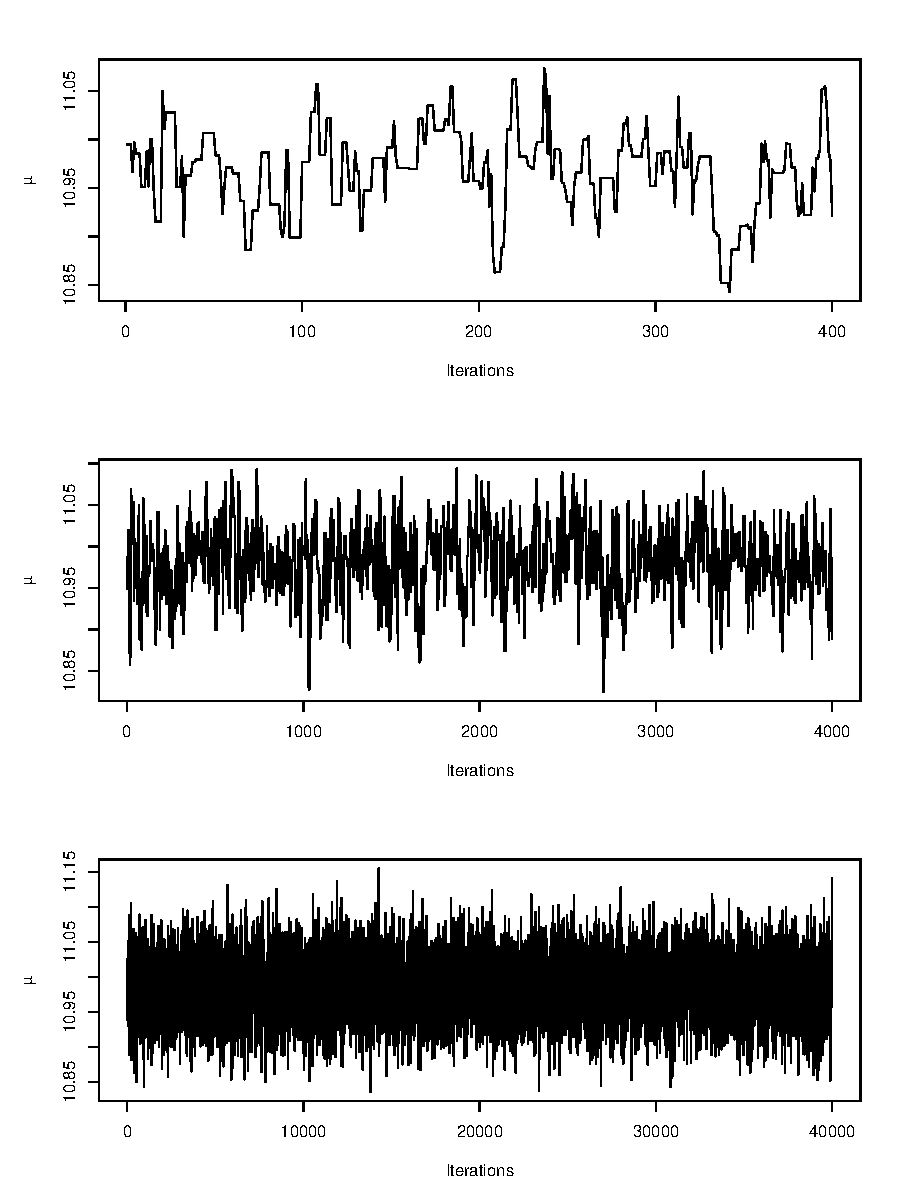
\includegraphics[scale=0.39]{figuras/trace_mu_mh.pdf}}}%
	\qquad
	\subfloat[Autocorrelação de $\mu$]{{
		\label{fig:acf_mu_mh}
		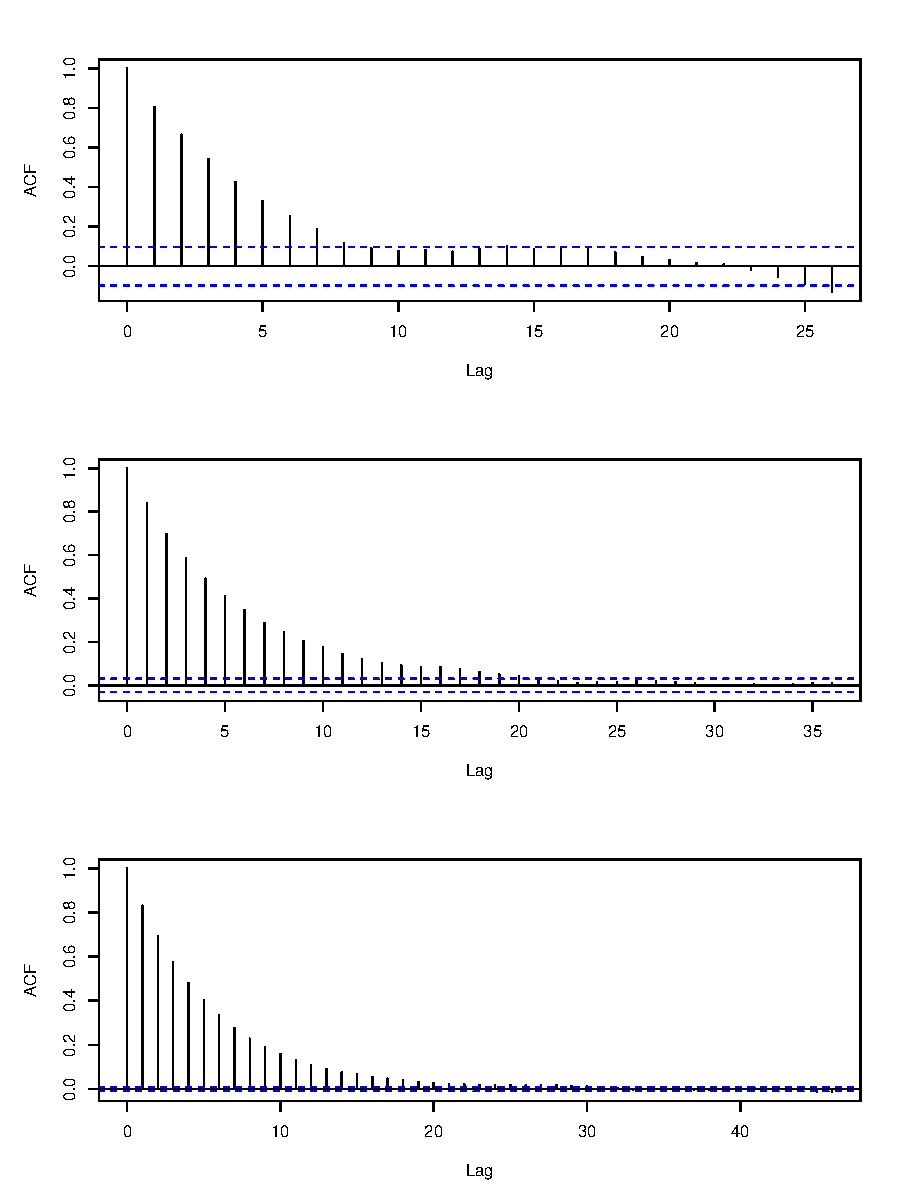
\includegraphics[scale=0.39]{figuras/acf_mu_mh.pdf}}}%
	\caption{Traço e autocorrelação da cadeia de $\mu$, $k = \{500, 5000, 50000\}$, respectivamente}%
\end{figure}

\begin{figure}[htb]
	\centering
	\subfloat[Traço de $\sigma^2$]{{
			\label{fig:trace_s2_mh}
			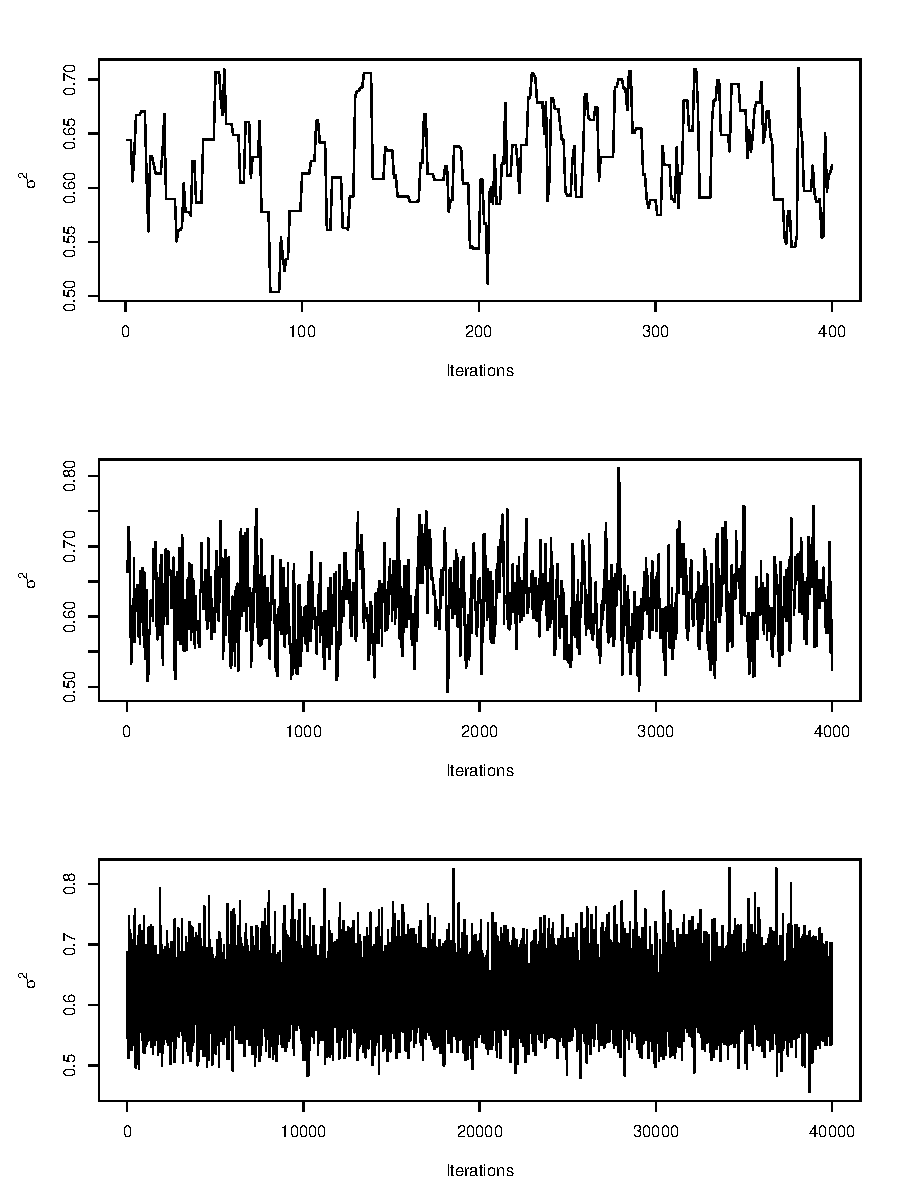
\includegraphics[scale=0.39]{figuras/trace_s2_mh.pdf}}}%
	\qquad
	\subfloat[Autocorrelação de $\sigma^2$]{{
			\label{fig:acf_s2_mh}
			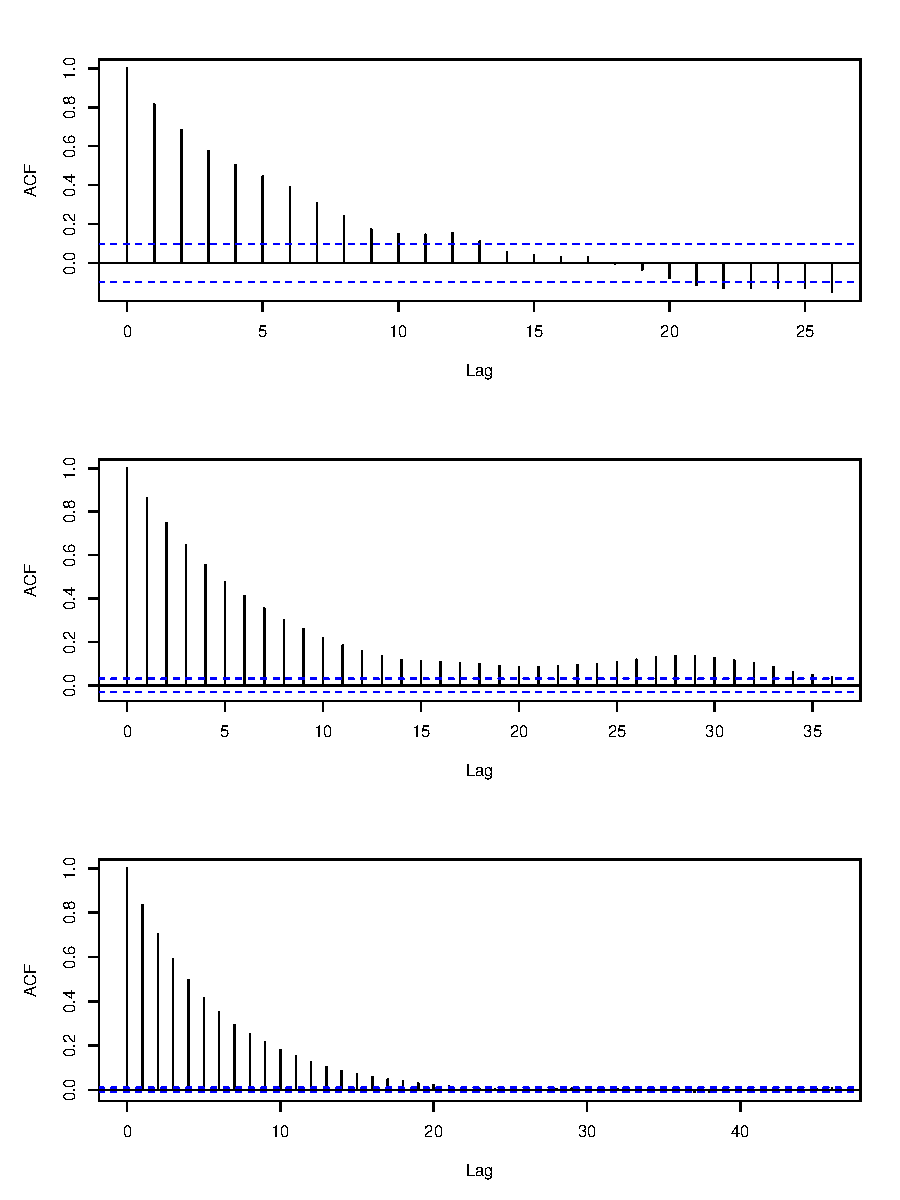
\includegraphics[scale=0.39]{figuras/acf_s2_mh.pdf}}}%
	\caption{Traço e autocorrelação da cadeia de $\sigma^2$, $k = \{500, 5000, 50000\}$, respectivamente}%
\end{figure}

\begin{figure}[htb]
	\centering
	\subfloat[Traço de $\nu$]{{
			\label{fig:trace_nu_mh}
			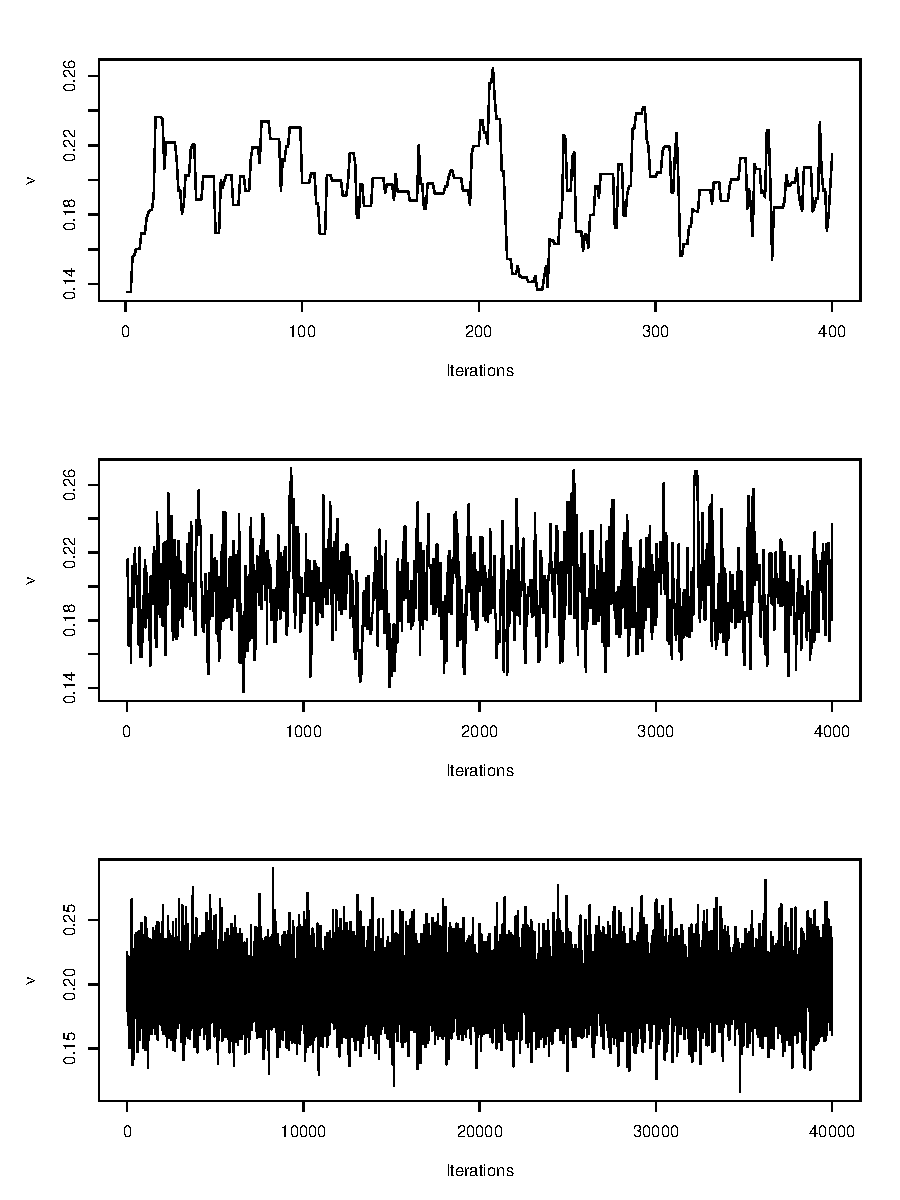
\includegraphics[scale=0.39]{figuras/trace_nu_mh.pdf}}}%
	\qquad
	\subfloat[Autocorrelação de $\nu^2$]{{
			\label{fig:acf_nu_mh}
			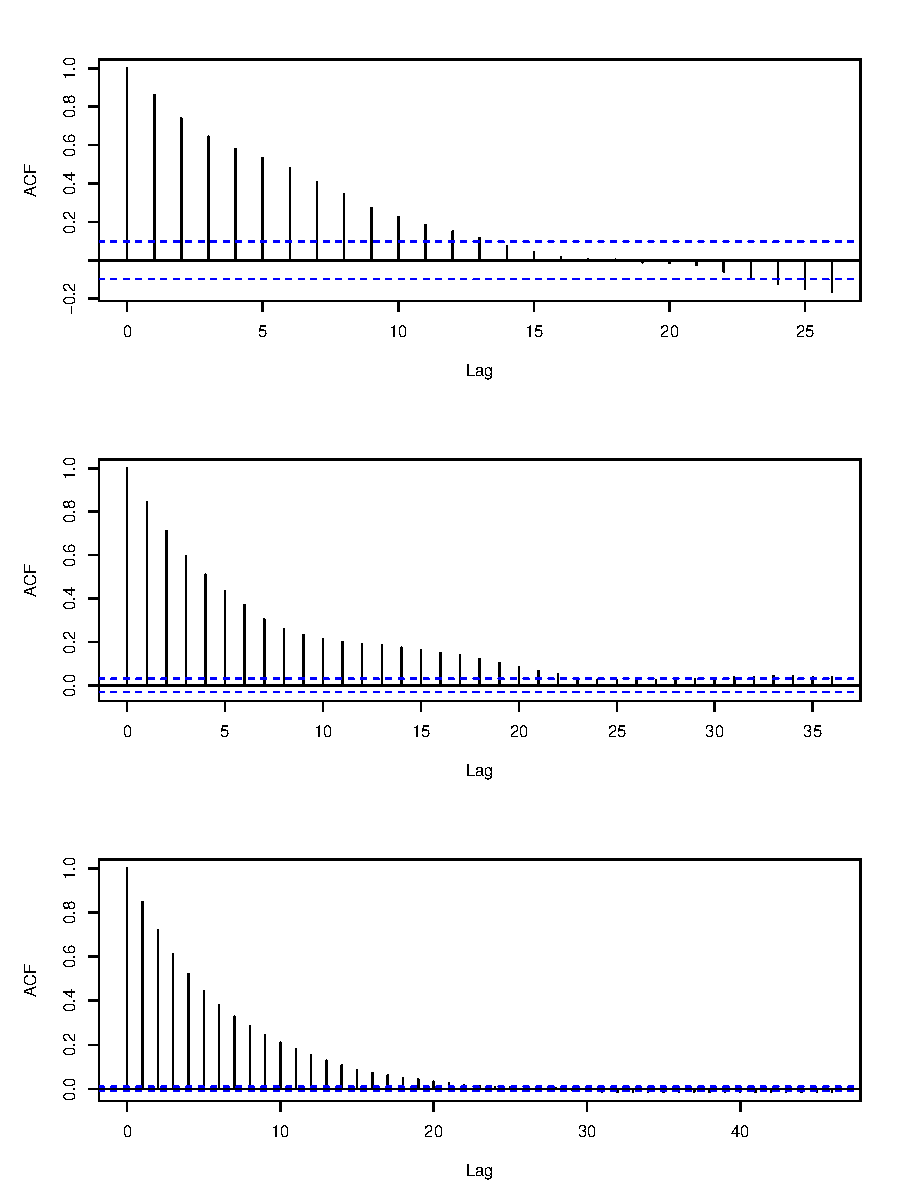
\includegraphics[scale=0.39]{figuras/acf_nu_mh.pdf}}}%
	\caption{Traço e autocorrelação da cadeia de $\nu^2$, $k = \{500, 5000, 50000\}$, respectivamente}%
\end{figure}

\end{document}